\documentclass[11pt]{article}
\usepackage[T1]{fontenc}
\usepackage[utf8]{inputenc}
\usepackage{lmodern}
\usepackage[margin=1.05in]{geometry}
\usepackage{amsmath,amssymb,amsthm,mathtools}
\usepackage{microtype,graphicx,booktabs,array,longtable}
\usepackage{enumitem}
\usepackage{tikz}
\usetikzlibrary{arrows.meta,positioning,calc,fit}
\usepackage[numbers,sort&compress]{natbib}
\usepackage[colorlinks=true,linkcolor=blue!45!black,citecolor=blue!45!black,urlcolor=blue!45!black]{hyperref}
\usepackage[capitalise,nameinlink,noabbrev]{cleveref}
\hypersetup{pdftitle={A counterexample to Hadwiger's conjecture},pdfauthor={OpenAI (construction), Édouard Bonnet and Codex (adaptation)},bookmarksdepth=2}
\setlength{\parskip}{0.18em}
\setlist{itemsep=0.18em,topsep=0.35em}
\makeatletter
\renewcommand*{\l@section}{\@dottedtocline{1}{0em}{2.3em}}
\makeatother
\numberwithin{equation}{section}
\newtheorem{theorem}{Theorem}[section]
\newtheorem{lemma}[theorem]{Lemma}
\newtheorem{proposition}[theorem]{Proposition}
\newtheorem{corollary}[theorem]{Corollary}
\newtheorem{conjecture}[theorem]{Conjecture}
\theoremstyle{definition}
\newtheorem{definition}[theorem]{Definition}
\newtheorem{construction}[theorem]{Construction}
\theoremstyle{remark}
\newtheorem{remark}[theorem]{Remark}
\newtheorem{example}[theorem]{Example}
\newcommand{\F}{\mathbb F_2}
\newcommand{\E}{\mathbb E}
\newcommand{\PP}{\mathbb P}
\newcommand{\R}{\mathbb R}
\newcommand{\N}{\mathbb N}
\newcommand{\cB}{\mathcal B}
\newcommand{\cX}{\mathcal X}
\newcommand{\cV}{\mathcal V}
\newcommand{\cE}{\mathcal E}
\newcommand{\cI}{\mathcal I}
\newcommand{\cK}{\mathcal K}
\newcommand{\cL}{\mathcal L}
\newcommand{\cR}{\mathcal R}
\newcommand{\cS}{\mathcal S}
\newcommand{\cD}{\mathcal D}
\newcommand{\cP}{\mathcal P}
\newcommand{\cQ}{\mathcal Q}
\newcommand{\cW}{\mathcal W}
\newcommand{\1}{\mathbf 1}
\DeclareMathOperator{\rank}{rank}
\DeclareMathOperator{\im}{im}
\DeclareMathOperator{\Span}{span}
\DeclareMathOperator{\GL}{GL}
\DeclareMathOperator{\Hom}{Hom}
\DeclareMathOperator{\End}{End}
\DeclareMathOperator{\Tr}{Tr}
\DeclareMathOperator{\supp}{supp}
\DeclareMathOperator{\diag}{diag}
\DeclareMathOperator{\cm}{cm}
\DeclareMathOperator{\had}{h}
\DeclareMathOperator{\Var}{Var}
\DeclareMathOperator{\TV}{TV}
\DeclareMathOperator{\codim}{codim}
\DeclareMathOperator{\id}{id}
\DeclareMathOperator{\Sym}{Sym}
\newcommand{\pair}[2]{\langle #1,#2\rangle}
\newcommand{\norm}[1]{\lVert #1\rVert}
\newcommand{\abs}[1]{\lvert #1\rvert}
\newcommand{\eps}{\varepsilon}
\newcommand{\trans}{^{\mathsf T}}
\ifdefined\pdfinfoomitdate\pdfinfoomitdate=1\fi
\ifdefined\pdftrailerid\pdftrailerid{}\fi


\title{A counterexample to Hadwiger's conjecture\\[.2em]
\large A proof using quadratic frames and linear partitions}
\author{Construction by OpenAI, September 2026\\
Adaptation by \'{E}douard Bonnet and Codex}
\date{November 27, 2026}
\begin{document}
\maketitle
\begin{abstract}
For arbitrarily large \(m\), we construct a graph on \(m\) vertices
with independence number at most 2 in which every connected matching has
fewer than \(m/100\) edges. Counting the branch sets of a complete minor
then shows that the Hadwiger number is smaller than the fractional
chromatic number. In particular, Hadwiger's conjecture is false.

The vertices are sampled from a finite probability space. A parity
identity ensures that among any three vertices some two are adjacent.
To rule out a large connected matching, we look for
two of its edges with no edge joining their endpoints. We bound the
probability of this event for two independent draws from a law on
edges satisfying explicit density bounds. The endpoints within either
draw may be dependent. Each of the four missing edges needs a pair of
witnesses with the same ambient image. Linear algebra over \(\F\)
supplies the witnesses' prescribed scalar values. A Fourier estimate
controls the probability that their images agree.

\end{abstract}
\begingroup
\small
\setlength{\parskip}{0pt}
\setcounter{tocdepth}{1}
\tableofcontents
\endgroup
\clearpage
\section{Introduction}\label{sec:introduction}

For a finite graph \(G\), write \(\alpha(G)\), \(\chi(G)\), and \(h(G)\)
for its independence number, chromatic number, and Hadwiger number.
Thus \(h(G)\) is the largest \(t\) for which \(G\) contains a \(K_t\)
minor.

Hadwiger's conjecture, formulated in 1943~\citep{hadwiger1943},
asserts that \(h(G)\ge\chi(G)\) for every finite nonempty simple
graph \(G\). We disprove it using graphs of independence number
at most 2.

Two disjoint edges are \emph{touching} if an edge joins their
endpoint sets. A \emph{connected matching} is a matching whose edges
are pairwise touching. Write \(\cm(G)\) for the maximum size of a connected matching in \(G\).

% lax begin Lax793645.Counterexample
\begin{theorem}\label{thm:main}
There are arbitrarily large integers \(m\) for which an \(m\)-vertex
finite simple graph \(G\) satisfies
\[
             \alpha(G)\le2
             \qquad\text{and}\qquad
             \cm(G)<\frac{m}{100}.
\]
\end{theorem}
% lax end

The connection to minors comes from the small branch sets of a
\(K_t\) minor. Its branch sets of size 2 form a connected matching,
and pairing its singleton branch sets gives more edges in the same
matching. Counting the vertices in the remaining branch sets gives
\[
                    h(G)\le\frac{|V(G)|+4\cm(G)+2}{3}
\]
(Proposition~\ref{prop:matching-minor}).

It is enough to compare this upper bound with the fractional chromatic
number. Write \(\mathcal I(G)\) for the independent sets of \(G\).
A fractional coloring assigns each \(I\in\mathcal I(G)\) a weight
\(w_I\ge0\) such that \(\sum_{I\ni v}w_I\ge1\) at every vertex \(v\).
The minimum total weight is \(\chi_f(G)\). Giving weight 1 to each
color class of an ordinary coloring shows that \(\chi_f(G)\le\chi(G)\).

% lax begin Lax793645.FractionalCounterexample
\begin{corollary}\label{cor:hadwiger}\label{cor:fractional-hadwiger}
There are finite nonempty simple graphs \(G\) of arbitrarily large
order \(m\) for which
\[
 h(G)<\frac{26m}{75}+\frac23
 <\frac m2\le\chi_f(G)\le\chi(G).
\]
Thus Hadwiger's conjecture and its weakening to fractional colorings
\(\chi_f(G)\le h(G)\) are false.
\end{corollary}
% lax end
% lax begin Lax793645Proofs.FractionalCounterexample.arbitrarily_large_fractional_counterexample
\begin{proof}
Summing the vertex constraints of any fractional coloring gives
\[
 |V(G)|\le\sum_{I\in\mathcal I(G)}|I|w_I
       \le\alpha(G)\sum_{I\in\mathcal I(G)}w_I.
\]
Hence \(\chi_f(G)\ge |V(G)|/\alpha(G)\). Apply
\Cref{thm:main} and the minor bound above, noting that
\(26m/75+2/3<m/2\) for \(m\ge5\).
% lax begin Lax793645Proofs.Counterexample.arbitrarily_large_hadwiger_counterexample
Since \(\chi_f(G)\le\chi(G)\), the same graphs satisfy \(h(G)<\chi(G)\).
% lax end
\end{proof}
% lax end

\citet[p.~148]{reedseymour1998} discussed the conjecture that every graph with no
\(K_{p+1}\) minor has a fractional \(p\)-coloring and proved a
\(2p\) bound in their result (1.3). They require rational weights
and coverage exactly 1 at each vertex. Such weights satisfy the
constraints above, so taking \(p=h(G)\) also disproves their formulation.

\subsection{Context}

Hadwiger's conjecture was proposed in 1943~\citep{hadwiger1943}.
Its restriction to graphs with independence number at most 2 is equivalent
to the assertion that every such graph of order \(m\) has a
\(K_{\lceil m/2\rceil}\) minor~\citep[Theorem~3.1]{pst2003}.
The general bound of Duchet and Meyniel~\citep{duchet1982} gives a minor
of order at least \(m/3\) in this case. Our examples have Hadwiger number
less than \(26m/75+2/3\).

F\"uredi, Gy\'arf\'as, and Simonyi~\citep{fgs2005} conjectured that a graph
with independence number two and order \(4t-1\) has a connected matching
of size \(t\). \Cref{thm:main} disproves this statement as well. Delete
at most 3 vertices to obtain order \(4t-1\); the connected matching
number does not increase. The result does not assert that the matching
number is sublinear. It leaves open the possibility of a smaller universal
positive linear lower bound.

The proof below is an exposition of the construction in the accompanying
Lean submission. It does not use the separate counterexample based on the
Colin de Verdi\`ere invariant~\citep{OpenAIColinDeVerdiereCounterexample2026}.



\subsection{How the proof works}

We first define a symmetric relation on a finite set. We call a related
pair a \emph{hole}. To obtain a graph, sample \(m\) elements of the set
independently and join two distinct sample positions if there is no hole
between their elements. The relation has no loops, so two positions
carrying the same element are adjacent. A parity argument excludes
triangles of holes and hence independent sets of size 3.

Call an ordered pair with no internal hole a \emph{unit}. It represents
an edge of the sample graph. Two units \emph{conflict} if all four pairs
between them are holes. Edges of a connected matching cannot conflict.

\begin{figure}[htbp]
\centering
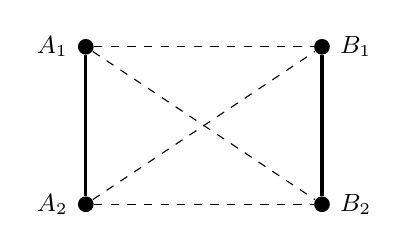
\begin{tikzpicture}[every node/.style={font=\small}]
\node[circle,fill=black,inner sep=2pt,label=left:$A_1$] (a1) at (0,1) {};
\node[circle,fill=black,inner sep=2pt,label=left:$A_2$] (a2) at (0,-1) {};
\node[circle,fill=black,inner sep=2pt,label=right:$B_1$] (b1) at (3,1) {};
\node[circle,fill=black,inner sep=2pt,label=right:$B_2$] (b2) at (3,-1) {};
\draw[very thick] (a1)--(a2); \draw[very thick] (b1)--(b2);
\draw[dashed] (a1)--(b1); \draw[dashed] (a1)--(b2);
\draw[dashed] (a2)--(b1); \draw[dashed] (a2)--(b2);
\end{tikzpicture}
\caption{The solid edges conflict when all four dashed pairs are holes.}
\label{fig:four-holes}
\end{figure}

Choosing an edge from a matching biases the choice of its endpoints.
A conflict estimate for four independent vertices would therefore be
insufficient. Theorem~\ref{thm:raw-supersaturation} gives a lower bound
for two independent units drawn from the same law. It allows dependence
within each unit and bounds how heavily its law can weight any vertex
or pair of vertices.

Here is how we witness a hole. Each raw vertex carries a linear
embedding on each edge of an auxiliary odd cycle. A point at a cycle
vertex has two images, one in each incident component. We call this
pair of images its \emph{key}. For each of the four proposed holes we
seek two short lists of points, one at either endpoint. If corresponding
keys agree, the sums of their point matrices have the same ambient
image. Further equations prescribe a linear functional on these sums.
We show that once the scalar equations hold, the remaining matrix
entries can be filled in without changing any images already fixed.

The lists at opposite ends of a hole are sampled independently before
we ask for their keys to agree. Such an equality is rare. To estimate
its probability we compare the two distributions of accepted keys.
Finite Fourier analysis lets us replace a distribution by its averages
on the cells of a partition given by linear equations. A character of
a tuple of keys factors into characters of its individual keys, so we
can test a whole list using information about individual points.

If the scalar equations have no solution, a linear relation determines
one of the recorded bits from the common key coordinates. This relation
holds for every point with those coordinates, which makes the prediction
an exact quadratic identity. When many units share a prediction, a
separate argument finds solutions on compatible pairs of units. Their
probability can be as small as order \(N^{-4}\). We bound the exceptional
probabilities under independent sampling before restricting to such pairs.

Finally, suppose every sample had a large connected matching. From each
matching select a short list of edges. With high probability it meets the set of
edges conflicting with any given unit whose conflicts occupy a substantial
fraction of the matching. Samples that supply
the same list then yield a law on edges under which two independent
draws conflict too rarely. This contradicts the lower bound.

\subsection{Conventions}

All vector spaces are over \(\F\). Probabilities and norms are real.
The polar form of \(q\) is \(\beta_q(v,w)=q(v+w)+q(v)+q(w)\).
We evaluate \(q\) on symmetric matrices by linearity, assigning
\(vv\trans\) the value \(q(v)\). These matrices span the symmetric
matrices.

The integer \(n\) tends to infinity. We write \(N=M_0n\) for the full
ambient dimension, with \(M_0\) a fixed even integer. The corresponding
dimension parameter in Lean is \(N/2\). All construction parameters are
fixed before \(n\). A bounded quantity is bounded independently of \(n\).

An \emph{orientation} specifies the two raw vertices of a unit in order.
At a fixed orientation a \emph{query} draws the parameters of its points.
We sometimes fix the images of prescribed directions, called \emph{pins}.
A \emph{leaf} carries the resulting conditional law together with the
images already fixed. In a mixture of leaves we retain the probability
of each leaf. Likewise, the measure of accepted keys has total mass equal
to the probability of acceptance.

\section{The hole relation and its tensor realization}\label{sec:geometry}

Three pairwise missing edges would give an independent set of size
three. We choose a relation that excludes such a triangle by parity.
Later we choose its linear maps so that four missing edges occur often
enough between two units.

\subsection{A triangle-free relation}

Let \(\cX\) and \(\cV\) be finite-dimensional vector spaces over
\(\F\). Fix a linear functional \(a\in\cX^*\) and a symmetric
bilinear form \(T\) on \(\cX\), and write
\[
 r(x)=a+T(x,\cdot)\in\cX^*.
\]
Let \(\Omega\) be a finite set. For each \(i\in\Omega\), suppose
we have an injective linear map \(U_i:\cX\to\cV\) and a linear
functional \(u_i\in\cV^*\).

% lax begin Lax793645.Holes
\begin{definition}\label{def:hole}
Two elements \(i,j\in\Omega\) have a \emph{hole} between them if
there exist \(\lambda_i,\lambda_j\in\cX\) such that
\begin{equation}\label{eq:hole-equations}
 \begin{gathered}
 U_i\lambda_i=U_j\lambda_j,\qquad
 u_jU_i=r(\lambda_i),\qquad u_iU_j=r(\lambda_j),\\
 a(\lambda_i)+a(\lambda_j)=1.
 \end{gathered}
\end{equation}
The middle two identities are identities of linear functionals on
the whole space \(\cX\).
\end{definition}
% lax end

Thus a hole has a shared vector in \(\cV\), one witness for it in
each copy of \(\cX\), and opposite values of \(a\) on the witnesses.
The functional identities make these requirements incompatible around
a triangle.

% lax begin Lax793645.TriangleFreeHoles
\begin{lemma}\label{lem:hole-triangle-free}
The hole relation is symmetric, has no loops, and is triangle-free.
\end{lemma}
% lax end
% lax begin Lax793645Proofs.Manuscript.TriangleFreeHoles.triangle_free
\begin{proof}
Symmetry follows by interchanging the endpoints.
A loop would have \(U_i\lambda_i=U_i\lambda_j\), hence
\(\lambda_i=\lambda_j\) by injectivity, contradicting the last
equation of \Cref{eq:hole-equations}.

Suppose that three distinct elements have holes on all three pairs.
For a directed incidence \(ij\), let \(x_{ij}\) be its witness at
\(i\). For distinct \(i,j,k\), evaluating the functional identity for
\(ij\) on \(x_{ik}\) gives
\[
 u_j(U_ix_{ik})=a(x_{ik})+T(x_{ij},x_{ik}).
\]
Sum over the six ordered choices of \((i,j,k)\).
For fixed \(j\), the two arguments on the left are equal by the
sharing equation for the remaining edge \(ik\), so they cancel.
For fixed \(i\), the two bilinear terms cancel by symmetry of \(T\).
The remaining sum is
\[
 \sum_{\{i,j\}}\bigl(a(x_{ij})+a(x_{ji})\bigr)=1+1+1=1,
\]
a contradiction.
\end{proof}
% lax end

Given any list \(o_1,\ldots,o_m\in\Omega\), form a graph \(G\)
on its \emph{positions}: two distinct positions are adjacent when
their elements have no hole. This gives a finite simple graph even
when elements repeat. Equal elements are adjacent because holes have
no loops. An independent triple of positions would therefore give
three distinct elements forming a hole triangle. Hence
\begin{equation}\label{eq:sample-independence}
 \alpha(G)\le2,\qquad \chi(G)\ge\lceil m/2\rceil.
\end{equation}

It remains to choose the finite set and its linear data so that a
random list also has no large connected matching. Two disjoint edges
fail to touch precisely when all four cross pairs are holes. The
distribution theorem in \Cref{sec:distributions} will force these
four-hole conflicts for the model constructed below.


\subsection{Points and the odd cycle}

Fix a large odd integer \(g\). Tags are the elements of \(\mathbb Z/g\mathbb Z\).
There is one component
\[
 e_l=\{l,l+1\}
\]
for each tag \(l\). We choose \(g\) after the initial pin budget, as
specified in Appendix~\ref{sec:parameters}. It does not grow with the graph.

The base coordinates have one constant coordinate and blocks
\[
 O_{l,t}\quad(l,t\in\mathbb Z/g\mathbb Z),\qquad S,\quad \#,\quad Z.
\]
Each block has \(n\) coordinates. At tag \(l\), only the ordinary blocks
\(O_{l,t}\) are allowed. The blocks \(S,\#,Z\) are shared by all tags.
We write \(F\) for the base vector space, including its constant coordinate.
A base point is \(\bar z=(1,z)\in F\). A point allowed at tag \(l\)
has zero coordinates in every \(O_{l',t}\) with \(l'\ne l\).

Labels are vectors \(s\in\F^b\). Set
\[
 \mathsf S=\F^{b+1},\qquad p_s=(1,s),\qquad
 B=\mathsf S\otimes F,\qquad v(s,z)=p_s\otimes\bar z.
\]
Later, \(S_0\) will denote a protected subspace of \(\mathsf S\).
The point matrix is \(v(s,z)v(s,z)\trans\).
Let \(W_l\) be the span of point matrices allowed at tag \(l\).
Let \(W_*\) be the corresponding span when all ordinary coordinates are
zero. Then \(W_l\cap W_{l'}=W_*\) for distinct tags. To see this, use
the ordinary affine point-matrix basis: its entries involve only coordinates
allowed at that tag. The entries common to two tags are exactly the shared
ones.

Define the space of profiles by
\[
 \cX=\left\{x:\ x_{e_l}=w_l+w_{l+1},\quad w_l\in W_l\right\}.
\]
Thus a point at tag \(l\) gives a profile, called an \emph{atom}, with its
point matrix on the two incident components and zero elsewhere.
We denote it by \(A(l,s,z)\). The kernel of \((w_l)_l\mapsto x\)
consists of constant tuples with value in \(W_*\): equality of consecutive
terms propagates around the cycle.

\subsection{Testers and the scalar form}

In each ordinary block and in \(S\), reserve \(2r_0\) coordinates.
Pair them and sum their products. These quadratic expressions define linear
functionals on point matrices, denoted by \(\eta_{l,t}\) and \(\eta_S\).
Write
\[
 \eta_O=\sum_{l,t}\eta_{l,t},\qquad \eta=\eta_O+\eta_S.
\]
All tester functionals ignore \(\#\) and \(Z\). Their matrices use the
constant selector coordinate. The polar rank of a sum of \(a\) disjoint
testers is \(2ar_0\).

Delete tag \(t\) from the cycle. The remaining path has the perfect matching
\[
 M_t=\{e_{t+1},e_{t+3},\ldots,e_{t+g-2}\}.
\]
Define linear functionals directly on the component matrices:
\begin{equation}\label{eq:cycle-functionals}
 a_t(x)=\sum_l\eta_{l,t}(x_{e_l}),\qquad
 a(x)=\sum_ta_t(x),\qquad
 b_t(x)=\sum_{e\in M_t}\eta_S(x_e).
\end{equation}
If \(x_{e_l}=w_l+w_{l+1}\), the private ordinary blocks and the matching
identity give
\[
 a_t(x)=\sum_l\eta_{l,t}(w_l),\qquad
 b_t(x)=\sum_{l\ne t}\eta_S(w_l).
\]
These formulas explain the definitions; no choice of representation is
needed to define the functionals.

The first part of the scalar form is
\[
 T^0(x,y)=a(x)a(y)+\sum_t\bigl(a_t(x)b_t(y)+b_t(x)a_t(y)\bigr).
\]
In particular \(T^0(x,x)=a(x)\).
For later use, put \(z_c(x)=\sum_{e\in M_c}x_e\).
Choose matrices \(L_j^c,R_j^c\), with \(1\le j\le J\), and define
\begin{equation}\label{eq:reduced-mixer}
 B^1(x,y)=\sum_{c,j}\pair{x_{e_c}}{L_j^c z_c(y)(R_j^c)\trans},
 \qquad T^1(x,y)=B^1(x,y)+B^1(y,x).
\end{equation}
Here \(\pair{A}{B}=\sum_{i,j}A_{ij}B_{ij}\). Set \(T=T^0+T^1\).
This form is symmetric and satisfies \(T(x,x)=a(x)\).
The matrices will be chosen in \Cref{sec:moments}. There are \(Jg\)
pairs of them.

The matching has a useful effect on atoms:
\begin{equation}\label{eq:matching-atom}
 z_c(A(l,s,z))=
 \begin{cases}v(s,z)v(s,z)\trans,&c\ne l,\\0,&c=l.\end{cases}
\end{equation}
Every tag other than \(c\) occurs exactly once in \(M_c\).
This is why a small mixer family suffices.

\subsection{Counting ordinary tester bits}

Put \(o_l(x)=\sum_t\eta_{l,t}(x_{e_l})\). Privacy of the ordinary
blocks gives
\[
 o_l(x)+o_{l+1}(x)=\eta_O(x_{e_l}),\qquad
 \sum_l o_l(x)=a(x).
\]
We need only the following support bound.
% lax begin Lax793645.OrdinaryTesterSupport
\begin{lemma}\label{lem:ordinary-support}
For every profile \(x\), \(|\supp o(x)|\le\sum_e\rank x_e\).
\end{lemma}
% lax end
% lax begin Lax793645Proofs.Manuscript.OrdinaryTesterSupport.ordinaryBit_support
\begin{proof}
If \(o_l(x)=1\), an ordinary entry owned by \(l\) is nonzero.
Both incident components contain that entry. Each such tag contributes
two incidences with nonzero components, and each component receives at
most two. Thus the support size is at most the number of nonzero
components, which is at most their total rank.
\end{proof}
% lax end

\subsection{One quadratic frame per component}

Choose a matrix \(E\) on \(B\) whose value on each point is \(\eta\).
It consists of the tester matrices and a correction \(E^\#\) supported
on \(\#\). The latter has zero value on a single point; its off-point
values will ensure binary mixing. Define \(q_E(v)=v\trans Ev\) for
\emph{every} \(v\in B\).

Let \(V=\F^{N/2}\oplus\F^{N/2}\), with
\[
 q_0(x,y)=x\cdot y,
 \qquad \beta_0(v,w)=q_0(v+w)+q_0(v)+q_0(w).
\]
At each component choose an injective linear map on
\(B\oplus\F^h\oplus\F^h\). Its restrictions are denoted by \(P,X,Y\).
They satisfy
\begin{equation}\label{eq:one-frame}
 q_0(Pv)=q_E(v),\qquad \beta_0(X_j,Pv)=0
 \quad(v\in B,\ 1\le j\le h).
\end{equation}
There are no other prescribed quadratic values or pairings on the channel
columns. The full list of primal and channel columns is independent.
The uniform law on these frames exists once \(N\) is sufficiently large;
\Cref{sec:frame-laws} proves this and the counting facts we need.

A raw vertex \(o\) is an independent choice of such a frame at every
component. Its law is \(\mu\), on a finite set \(\Omega_n\).
Let \(\cV\) be the product of the ambient symmetric-matrix spaces. Define
\[
 (U_ox)_e=P_ex_eP_e\trans.
\]
The quadratic form
\[
 v\longmapsto\sum_{j=1}^h\beta_0(X_{e,j},v)\beta_0(Y_{e,j},v)
\]
defines a linear functional on symmetric matrices. Sum it over the
components to obtain \(u_o\in\cV^*\).
A left inverse to each \(P_e\) proves that \(U_o\) is injective.
Equation \eqref{eq:one-frame} gives \(u_oU_o=0\).
We use these maps in Definition~\ref{def:hole}.

The ambient functional defined by \(q_0\) satisfies
\[
 q_0[P_ex_eP_e\trans]=\eta(x_e)\quad(x_e\in W_l+W_{l+1}).
\]
Square brackets denote evaluation on a symmetric matrix. Therefore
\(U_ox=U_{o'}y\) implies equality of the component tester values:
\begin{equation}\label{eq:common-image-tester}
 U_ox=U_{o'}y\quad\Longrightarrow\quad\eta(x_e)=\eta(y_e)\quad\text{for every }e.
\end{equation}

All coefficient dimensions are \(O(n)\), with fixed implied constants.
Counting the entries of the component frames gives
\begin{equation}\label{eq:raw-space-size}
 \log_2|\Omega_n|=O(N^2).
\end{equation}
For the graph transfer we use
\[
 D=8000,\qquad M=2^{1000},\qquad m=2^{2000N},\qquad
 \varepsilon_N=2^{-200N}.
\]
The remaining choices, including \(h=1000r_0\) and \(M_0\), are made
in the order recorded in Appendix~\ref{sec:parameters}.

\section{From supersaturation to a finite graph}\label{sec:distributions}

A \emph{unit} is an ordered pair of raw vertices with no hole between its endpoints.
The endpoints of a unit may be dependent.
When two units are sampled independently, their four endpoints need not be independent within either unit.
The event of interest is that all four cross pairs have holes, as in \Cref{fig:four-holes}.

% lax begin Lax793645.FourHoles
\begin{theorem}[Raw supersaturation]\label{thm:raw-supersaturation}
For the construction parameters specified in \Cref{sec:geometry,sec:parameters}, for all sufficiently large \(n\), every probability law \(\sigma\) on units satisfying
\begin{equation}\label{eq:raw-law-caps}
 \sigma_1\le M\mu,\qquad \sigma_2\le M\mu,\qquad
 \sigma\le 2^{DN}\mu^2
\end{equation}
gives probability at least \(2^{-200N}\) that two independent units have all four cross holes.
The inequalities in \Cref{eq:raw-law-caps} are pointwise inequalities of measures on the finite raw spaces.
\end{theorem}
% lax end

The proof of \Cref{thm:raw-supersaturation} occupies the subsequent sections and is completed in \Cref{sec:rare-overlap}.
We prove its implication for graphs here. The frame estimates and the preparation of an admissible unit law begin in \Cref{sec:frame-laws}.

\subsection{A finite exposure potential}

Join two raw units when all four cross pairs are holes. The resulting
conflict graph has no loops. Write $q=\mu^2$,
$\kappa=2^{DN}$ and $\varepsilon=2^{-200N}$.
For $\gamma>0$ and an integer $b>0$ with $\kappa\le2^b\gamma$, put
\[
 \Phi(\sigma)=\sum_{i=0}^{b-1}\sum_x
      \min\{\sigma(x),2^i\gamma q(x)\}.
\]
Every summand indexed by $i$ has total at most one, so
$0\le\Phi(\sigma)\le b$ for every probability law $\sigma$.

% lax begin Lax793645.ClippedExposure
\begin{lemma}[Clipped exposure]\label{lem:clipped-exposure}
Let $(Y,X)$ have both marginals $\sigma$ and never consist of
conflicting units. Write $\tau_y$ for the conditional law of $X$
given $Y=y$. If $\sigma\le\kappa q$ on a set $A$, then
\[
 \Phi(\sigma)-\E_Y\Phi(\tau_Y)
 \ge \frac{(\sigma\otimes\sigma)(\text{conflict}\cap A^2)-\gamma}{2}.
\]
The potential drop is always nonnegative, without any assumption on $A$.
\end{lemma}
% lax end
% lax begin Lax793645Proofs.Manuscript.ClippedExposure.dyadic_exposure_joint
\begin{proof}
For each $x$ and each threshold $a=2^i\gamma$, the identity
$\E_Y\tau_Y(x)=\sigma(x)$ gives
\[
 \E_Y\min\{\tau_Y(x),aq(x)\}
 \le\min\{\sigma(x),aq(x)\}.
\]
Indeed the left side is separately bounded by both entries of the
minimum. Let $p_x$ be the probability that $Y$ conflicts with $x$. On that event,
$\tau_Y(x)=0$. If $\gamma q(x)\le\sigma(x)\le\kappa q(x)$,
choose a threshold with $aq(x)\le\sigma(x)\le2aq(x)$. The drop
at this coordinate and threshold is at least
$p_xaq(x)\ge p_x\sigma(x)/2$. Coordinates below $\gamma q(x)$
have total mass at most $\gamma$. Sum over $x\in A$ and discard
all other nonnegative drops. Restricting the first unit to $A$ can
only decrease the conflict probability.
\end{proof}
% lax end

\subsection{Sampling repeatedly from a matching}

% lax begin Lax793645.MatchingExposure
\begin{proposition}\label{prop:raw-to-graph}
Assume \Cref{thm:raw-supersaturation} for a sufficiently large $n$.
There is a sample of $m=2^{2000N}$ raw vertices whose graph satisfies
\[
 \alpha(G)\le2,\qquad \cm(G)<m/100.
\]
\end{proposition}
% lax end
% lax begin Lax793645Proofs.Manuscript.MatchingExposure.transfer_scales
\begin{proof}
Suppose instead that every sample has a touching matching of size
$k=\lceil m/100\rceil$. Choose one such matching deterministically
for each sample, and orient its edges arbitrarily. Given the sample,
draw repeatedly and independently from these $k$ oriented edges.
Two emissions never conflict, even if they are the same edge.
The hidden state is the original sample, with law $\mu^m$.

After any history $h$, let $\sigma_h$ be the law of the next emitted
unit under the posterior law of the hidden sample. Two future
emissions have both marginals $\sigma_h$ and never conflict.
The law after observing $y$ is the conditional second marginal
required by \Cref{lem:clipped-exposure}.

Define
\[
 S_h=\{x:(\sigma_h)_1(x)>M\mu(x)/4
               \text{ or }(\sigma_h)_2(x)>M\mu(x)/4\},
 \qquad
 E_h=\{x:\sigma_h(x)>\kappa q(x)/4\}.
\]
Summing each density excess gives
$\mu(S_h)\le8/M$ and $q(E_h)\le4/\kappa$.
Let $A_h$ consist of units avoiding $S_h$ at both endpoints and
avoiding $E_h$, and set $\alpha_h=\sigma_h(A_h)$.
If $\alpha_h\ge1/4$, the normalized restriction to $A_h$ satisfies
all three caps in \Cref{eq:raw-law-caps}. Raw supersaturation then gives
\[
 (\sigma_h\otimes\sigma_h)(\text{conflict}\cap A_h^2)
 \ge\varepsilon\alpha_h^2\ge\varepsilon/16.
\]
Use $\gamma=\varepsilon/32$. The drop $D_h$ in the potential is at
least $\varepsilon/64$ on these histories and is always nonnegative.
Since $\alpha_h\le1$, in all cases
\begin{equation}\label{eq:exposure-retention}
 D_h\ge\frac{\varepsilon}{48}(\alpha_h-1/4).
\end{equation}

Take $L=2^{400N}$ exposure steps and $s=\lfloor k/5\rfloor$.
There are at most $(|\Omega_n|^2+1)^L$ histories of length at most
$L$: this follows by induction from the recursion that either stops
or appends one unit. Each $S_h,E_h$ is a deterministic set in the raw
space. The iid sampling bounds therefore apply before any exposure.
A union bound shows that the probability of a raw sample having,
for some such history, $s$ positions in $S_h$ or $s$ disjoint
position pairs in $E_h$ is at most
\begin{equation}\label{eq:exposure-exceptions}
 \Delta=(|\Omega_n|^2+1)^L
 \left[2^m(8/M)^s+m^{2s}(4/\kappa)^s\right].
\end{equation}
Call this fixed event of raw samples bad. On a sample outside it,
at most $2(s-1)$ edges of the chosen matching fail the restrictions
for any history. Since $4s\le k$, its emission law gives $A_h$
probability at least $1/2$.

Let $B_h$ be the posterior probability of the fixed bad event.
Averaging the preceding bound under the original posterior gives
$\alpha_h\ge1/2-B_h$. The posterior probability $B_h$ is a
martingale: averaging its values after the next observation returns
its current value. Thus \eqref{eq:exposure-retention} and a finite
tree telescope imply
\[
 b\ge L\left(\frac{\varepsilon}{192}
                  -\frac{\varepsilon}{48}\Pr(\text{bad})\right).
\]
No posterior law has been conditioned on the complement of the bad event.

Here $D=8000$, $M=2^{1000}$ and $m=2^{2000N}$.
We may take $b=8200N+6$, so $\kappa\le2^b\gamma$.
By \Cref{eq:raw-space-size}, for all sufficiently large $N$,
\[
 (|\Omega_n|^2+1)^L\le2^{m/2},\qquad m\le550s.
\]
The two summands in \eqref{eq:exposure-exceptions}, including this
history factor, are each at most $2^{-m/4}$. For the first, compare
$m/2+m-997s$ with $-m/4$; for the second, compare
$m/2+(2-4000N)s$ with $-m/4$. Consequently $\Delta<1/8$.
But $L\varepsilon=2^{200N}>384b$ for large $N$, contradicting
the telescope. The required sample exists. Finally,
$\alpha(G)\le2$ holds for every sample by \Cref{lem:hole-triangle-free}.
\end{proof}
% lax end

\subsection{The clique-minor bound}

\Cref{prop:raw-to-graph} supplies the required bound on connected
matchings once raw supersaturation is proved. The next counting
argument converts that bound into the clique-minor estimate used in
the introduction.

The following elementary estimate counts small branch sets, in the
same connected-matching approach used by Cambie~\citep{cambie2021}.
Its deliberately coarse bound holds for every finite graph.

% lax begin Lax793645.MatchingMinorBound
\begin{proposition}\label{prop:matching-minor}
For every finite nonempty graph \(G\) of order \(m\),
\[
 \had(G)\le\frac{m+4\cm(G)+2}{3}.
\]
In particular, if \(\alpha(G)\le2\) and \(\cm(G)<m/100\), then
\[
 \had(G)<\frac{26m}{75}+\frac23<\frac m2\le\chi(G)
 \qquad(m\ge5).
\]
\end{proposition}
% lax end
% lax begin Lax793645Proofs.HadwigerMatching.hadwiger_matching_bound
\begin{proof}
Consider a complete-minor model with \(b\) branch sets.
Let \(s\) of them be singletons and \(e\) have two vertices.
Each two-vertex branch is an edge.
The singleton vertices form a clique, so pairing them gives \(\lfloor s/2\rfloor\) more edges.
All these edges together form one touching matching: their vertex sets are disjoint, and adjacency of the original branches guarantees every required contact.
Writing \(c=\cm(G)\), we obtain
\[
 c\ge e+\lfloor s/2\rfloor,\qquad s\le2(c-e)+1.
\]
Every remaining branch has at least 3 vertices, whence
\[
 m\ge s+2e+3(b-s-e)=3b-2s-e.
\]
Combining the inequalities gives
\[
 3b\le m+2s+e\le m+4c-3e+2\le m+4c+2.
\]
Maximize over all complete-minor models.
For the final assertion, every color class has at most 2 vertices when \(\alpha(G)\le2\), so \(\chi(G)\ge m/2\).
Combine this with \(c<m/100\) and \(26m/75+2/3<m/2\) when \(m\ge5\).
\end{proof}
% lax end

\section{Counting frames and fixing images}\label{sec:frame-laws}

The cost of prescribing frame images depends on the number of independent
directions observed. We count their possible images first.

\subsection{Quadratic Gram data}

For vectors \(v_1,\ldots,v_a\), their quadratic Gram data consist of
\(q_0(v_i)\) and \(\beta_0(v_i,v_j)\), for \(i<j\).
There are \(a(a+1)/2\) entries. Each diagonal entry records a quadratic value.

% lax begin Lax793645.QuadraticFrameCounts
\begin{lemma}\label{lem:quadratic-frame-count}
Suppose \(v_1,\ldots,v_a\) are independent in a hyperbolic space of
full dimension \(N\). For any prescribed \(b_1,\ldots,b_a,q\), the
number of vectors \(v\) satisfying
\[
 \beta_0(v_i,v)=b_i,\qquad q_0(v)=q
\]
is \(2^{N-a-1}(1+O(2^{a-N/2}))\). The number of such vectors outside
the previous span depends only on the quadratic Gram data and the
prescribed entries. Consequently every partial isometric embedding has
the same number of completions.
\end{lemma}
% lax end
% lax begin Lax793645Proofs.Manuscript.QuadraticFrameCounts.quadratic_column_mass
\begin{proof}
Nondegeneracy makes the polar equations independent. Their solution set
has size \(2^{N-a}\). The quadratic Gauss sum on that set is
\[
 2^{N/2-a}\sum_{t\in\F^a}
 (-1)^{q_0(\sum_i t_iv_i)+t\cdot b}.
\]
To obtain this identity, expand each polar equation as
\(\frac12\sum_{t_i\in\F}(-1)^{t_i(\beta_0(v_i,v)+b_i)}\),
then translate \(v\) by \(\sum_i t_iv_i\) in the hyperbolic Gauss sum.
The sum has absolute value at most \(2^{N/2}\). It is the number of
solutions with quadratic value 0 minus the number with value 1. Their
sum is \(2^{N-a}\), which gives the asserted count for either value.

A vector in the old span is \(\sum_i t_iv_i\). Whether it satisfies the
new equations is determined by the old Gram data. Thus the number excluded
by independence is determined by those data as well. In particular,
two lists with the same Gram data admit equally many choices for their
next independent vector. Complete the first list to a basis. At each step
there is a matching choice for the second list, since the first has at
least one choice. The linear map between the resulting bases preserves
the quadratic form. This uses the exact count at every dimension.
\end{proof}
% lax end

For \(a\le N/4\), it follows that a uniform list of ambient vectors has
prescribed independent quadratic Gram data with probability
\begin{equation}\label{eq:quadratic-gram-count}
 2^{-a(a+1)/2}\bigl(1+O(a2^{a-N/2})\bigr).
\end{equation}
The same count gives the frames in \eqref{eq:one-frame}. If
\(N\ge 2a+4\), at least \((2^{N-a}-2^{N/2})/2\) vectors realize
any prescribed next entries. This exceeds \(2^a\), the size of the
previous span. Appending independent columns therefore gives an embedding
with the required Gram data.

The frame law prescribes only part of the full Gram data. Sum the completion
counts over the unspecified entries. This shows that an independent list
of primal directions has exactly the uniform image law with its prescribed
quadratic Gram data. It also gives the following estimates, used repeatedly.
For every fixed \(\xi>0\), by choosing \(M_0\) large enough, any consistent
prescription of \(t\) new image directions has raw probability at most
\begin{equation}\label{eq:image-cost}
 2^{-(1-\xi)tN}.
\end{equation}
The bound is uniform over the already stored bounded set of directions.
For free entries of a bounded cross table, every consistent assignment
has probability \(2^{-c+o(N)}\), where \(c\) is the number of independent
scalar equations. A prescribed kernel must be counted separately from
these Gram equations. We do that explicitly in \Cref{sec:histograms}.

\subsection{Leaves with stored images}

A \emph{pin} specifies the exact images of a coefficient subspace under
the unit's frame maps. A \emph{leaf} is a conditional law together with
its pins. We require the pin space to be closed under projection onto the
primal and the two channel blocks at each of the two endpoints.
There are six projections.

For a leaf, a further exact-image event has \emph{new rank} \(t\) if it
prescribes \(t\) coefficient directions independent modulo the stored
ones. Call the leaf \(\zeta\)-spreading if every such event has probability
at most \(2^{-(1-\zeta)tN}\). Only the bounded ranks used in the subsequent
queries are needed.

% lax begin Lax793645.ClosedPins
\begin{lemma}[Closed pins]\label{lem:closed-peeling}
From a unit law with a fixed exponential density cap one can retain
at least half its mass as a mixture of spreading leaves. Their total pin
dimension on each leaf has a bound independent of \(n\). The pins
may be required to be closed under the six block projections. Further
restriction to a set of mass \(2^{-o(N)}\) allows another such decomposition,
with a larger fixed pin budget and twice the original spreading error.
\end{lemma}
% lax end
% lax begin Lax793645Proofs.Manuscript.ClosedPins.one_first_leaves
\begin{proof}
If a leaf violates spreading, condition on a violating exact-image event
of new rank \(t\). Close its coefficient space under the block projections.
Let \(u\) be the total new dimension after closure, including the
original \(t\) directions. Each direction has at most 6 projections, so
\(t\le u\le6t\). There are at most \(2^{(u-t)N}\) ways to specify the
remaining images. Some choice has conditional probability at least
\(2^{-(u-t)N}\). The whole step thus has mass at least
\[
 2^{-(1-\zeta)tN}2^{-(u-t)N}
 \ge2^{-(1-\zeta/6)uN}.
\]
The raw image bound \eqref{eq:image-cost}, with \(\xi<\zeta/6\), charges
strictly more for the same stored directions. After total new dimension
\(k\), the likelihood ratio has gained at least
\(2^{(\zeta/6-\xi)kN}\). The initial density cap bounds this ratio.
Choose the pin budget larger than the cap exponent divided by
\(\zeta/6-\xi\). No branch of this procedure can exceed that budget.

To form a mixture, keep a residual subset of the original finite law.
While it has mass at least \(1/2\), normalize it and run the preceding
procedure until a spreading leaf is obtained. Remove that leaf from the
residual set and record its original probability. The residual law has
at most twice the initial density cap, so one pin budget works at every
iteration. Each removal has positive mass. Finiteness makes the process
terminate, and the recorded leaves together retain at least \(1/2\) of
the law. Their weights are the actual removed masses.

For the second assertion, start with the old pins and allow a fixed reserve
of new directions. Restricting by mass \(2^{-o(N)}\) adds only \(o(N)\)
to the logarithm of the density cap. That cost fits in the reserve for
large \(n\). The same construction, with twice the spreading error,
gives the new leaves.
\end{proof}
% lax end

Let \(K\) bound the total pin dimension. Write \(P_{i,e}\le B\) for the
primal pins at endpoint \(i\), component \(e\). Closure under the block projections ensures that the images of these
primal directions are among the stored data.
For a subspace \(D\), write
\[
 D^{(2)}=\Span\{vv\trans:v\in D\}.
\]
The effective profiles at endpoint \(i\) form
\begin{equation}\label{eq:effective-space}
 C_i=\{x\in\cX:x_e\in P_{i,e}^{(2)}\text{ for every }e\}.
\end{equation}
They have dimension at most \(K^2\), and every such profile has total
component rank at most \(K\). Choose a basis on each leaf. Evaluations
on that basis will be part of the finite status of a query.

Later restrictions preserve the old pins and effective profiles. The
retained mass \(\theta_n\) is bounded below by a positive constant in
Proposition~\ref{prop:status-preparation}. We use this bound in the final probability
comparison.

\section{Witness vectors and mixing matrices}\label{sec:moments}

A witness must be distinguishable from the directions whose images we
have fixed. To see how to choose it, regard a vector of
\(B=\mathsf S\otimes F\) as a matrix with rows indexed by selector
coordinates and columns indexed by base coordinates. A single point
\(p_s\otimes\bar z\) has rank 1 as such a matrix. We will also encounter
a different rank, that of a symmetric matrix acting on \(B\) itself.
The next two lemmas relate the two descriptions.

Write \(\mathsf F=F\), and let \(W\) be the span of the point matrices
on \(B\), allowing every tag. The linear forms \(\epsilon_{\mathsf S}\)
and \(\epsilon_{\mathsf F}\) read the constant coordinate in each factor.

\subsection{The span of the point matrices}

% lax begin Lax793645.AffinePointMatrices
\begin{lemma}\label{lem:base-moments}
The span of $(1,z)(1,z)\trans$ consists precisely of symmetric matrices
$Z$ satisfying $\operatorname{diag}Z=Z\epsilon_{\mathsf F}$.
Consequently $W$ is the tensor product of the corresponding affine
point-matrix spaces on $\mathsf S$ and $\mathsf F$. Its tensors are
separately symmetric in the selector and base indices and satisfy the
Boolean diagonal identity in each factor.
\end{lemma}
% lax end
% lax begin Lax793645Proofs.Manuscript.AffinePointMatrices.mem_span_pointSquare_iff
\begin{proof}
Write \(P(z)=(1,z)(1,z)\trans\). Every \(P(z)\) is symmetric and has
\(P(z)_{ii}=P(z)_{i0}\). Conversely, let \(Z\) have these properties.
Choose an ordinary coordinate \(i\). Set \(u_i=1\) and
\(u_j=Z_{ji}\) for the other ordinary coordinates. The matrix
\[
 Z-P(u)-(Z_{ii}-1)P(e_i)
\]
has zero row and column at \(i\). It still satisfies the same identities,
and previously cleared rows and columns remain zero. Repeat at the remaining
coordinates. The matrix left at the constant coordinate is a multiple of
\(P(0)\). This proves the span assertion.
% lax begin Lax793645Proofs.Manuscript.AffinePointMatrices.affineTensor_identities
The tensor-product assertion follows because the selector
and base points vary independently. The identities in another basis
use the coordinates of $\epsilon_{\mathsf S},\epsilon_{\mathsf F}$.
% lax end
\end{proof}
% lax end

% lax begin Lax793645.SelectorConfinement
\begin{lemma}\label{lem:selector-confinement}
If $w$ is a symmetric matrix on $\mathsf S\otimes\mathsf F$, separately
symmetric in its two pairs of indices, and $\rank w\le r$, then
\[
 \operatorname{col}(w)\subseteq U\otimes\mathsf F
 \quad\text{for some }U\subseteq\mathsf S,\quad \dim U\le r^2.
\]
Consequently each vector in the column space has rank at most \(r^2\)
when reshaped as a matrix with one row per selector coordinate.
\end{lemma}
% lax end
% lax begin Lax793645Proofs.Manuscript.SelectorConfinement.selector_confinement
\begin{proof}
For a column of the tensor matrix indexed by $(b,j)$, reshape it as the
matrix $C_{ai}=w_{(a,i),(b,j)}$. Separate symmetry gives
$C_{ai}=w_{(a,j),(b,i)}$, so $C$ is a submatrix of $w$ and has rank
at most $r$. Choose at most $r$ columns spanning the original column space.
The sum of their reshaped column spaces has dimension at most $r^2$
and contains every selector slice.
\end{proof}
% lax end


\subsection{Protected subspaces}

Fix the pin budget \(K\) and an upper bound \(t_* =28\) for the number of
selected atoms. Choose
\[
 R\ge4(K+t_*),\qquad q_*=R^2+t_*.
\]
The extra room in \(R\) covers the joint obstruction at both endpoints.
In each primal pin space consider the span of the vectors whose rank
after reshaping is at most \(q_*\). Choose a basis of this span from
among those vectors. Let \(S_0\) be the sum of the column spaces of
the reshaped basis vectors. For \(F_0\), take the sum of the row spaces
of a basis of each \emph{whole} pin space. Take these sums over the
components of one endpoint, so the same \(S_0,F_0\) serve all its
components. If \(P_0\) bounds the sum of the pin dimensions, then

\begin{equation}\label{eq:label-budget}
 \dim S_0\le q_*P_0,\qquad \dim F_0\le(b+1)P_0.
\end{equation}
Set
\[
 D_0=S_0\otimes F_0,\qquad
 L=S_0\otimes\mathsf F+\mathsf S\otimes F_0.
\]
Every pin vector lies in \(L\). Every pin vector with reshaped rank at
most \(q_*\) lies in \(D_0\). The first bound in
\eqref{eq:label-budget} is independent of \(b\), and the second is independent
of \(n\).

% lax begin Lax793645.SelectedAtoms
\begin{lemma}\label{lem:protected-atoms}
Let $k_i=p_i\otimes v_i$, $1\le i\le t$, where
$\epsilon_{\mathsf S}(p_i)=\epsilon_{\mathsf F}(v_i)=1$.
Suppose the $p_i$ are independent modulo $S_0$ and the $v_i$ are
independent modulo $F_0$. Put $A=\operatorname{span}\{k_i\}$.
Then $A\cap L=0$. If $w\in W$ and
\[
 w\in(D_0+A)\otimes B+B\otimes(D_0+A),
\]
then
\[
 w=\sum_i c_i k_i k_i\trans+w_0,\qquad w_0\in L\otimes L.
\]
\end{lemma}
% lax end
% lax begin Lax793645Proofs.Manuscript.SelectedAtoms.tensor_atom_isolation
\begin{proof}
Extend bases of $S_0,F_0$ by the selected vectors and then to full bases.
The selected simple tensors occupy distinct diagonal positions outside
the rows and columns belonging to $L$, proving $A\cap L=0$.
An entry of $w$ must have an index in $D_0$ or at a selected position.
Separate symmetry moves the entry between $p_i\otimes v_i$ and
$p_a\otimes v_b$ to that between $p_i\otimes v_b$ and $p_a\otimes v_i$.
It is zero unless $a=i$ or $b=i$. If $a=i,b\ne i$, the diagonal entry
at $p_i\otimes v_b$ is zero. Its base diagonal identity has just one
potentially nonzero term, with coefficient
$\epsilon_{\mathsf F}(v_i)=1$, so that term is zero too.
The selector identity treats the other case. Each selected row and
column therefore has only its diagonal entry. Subtract these point
matrices. Every remaining entry has a $D_0$ index. If its other index
were outside $L$, separate symmetry would put both indices outside
$D_0+A$, forcing zero. Thus the residual tensor lies in $L\otimes L$.
\end{proof}
% lax end


A span of dimension \(d\) contains at most \(2^d\) affine selector vectors.
Thus the exclusions needed to choose the selectors independently modulo
\(S_0\) have a bound fixed before \(b\). Include the other finite label
exclusions used below in a budget \(B_{\rm exc}\), and choose
\begin{equation}\label{eq:selector-size}
 B_{\rm exc}<2^{b-2},\qquad 3B_{\rm exc}<2^b.
\end{equation}
When several lists are chosen, the exclusion budget includes all previously
chosen selectors. It is deliberately larger than needed for one list.

Base independence uses the free block \(Z\). Conditional on earlier point
parameters, a subspace of dimension at most \(\dim F_0+t_*\) contains at
most \(2^{\dim F_0+t_*}\) of the possible \(Z\)-vectors. Hence, at every
orientation, failure of independence modulo \(F_0\) has probability at most
\begin{equation}\label{eq:base-rejection}
 \delta_n=t_*2^{\dim F_0+t_*-n}=2^{-n+O(1)}.
\end{equation}
This probability is conditional on the orientation, and the bound is
the same for every orientation. Discarding these inputs therefore costs
at most \(\delta_n\) under any mixture of orientations.

\subsection{The input laws}

At tag \(l\), a generic query draws all its allowed coordinates
uniformly and independently. A shared point is obtained by setting its
ordinary coordinates to zero. We use shared points when evaluating
identities that hold for every generic point. Occasionally we prescribe
the few coordinates on which specified testers depend. Their number is
fixed, so the event has probability bounded below independently of \(n\).

The diagonal bit of an atom is \(q=\eta(vv\trans)\). Its role bit is
\(a(A)\).

Together with these bits, a query can record the individual
tester values and the evaluations \(T(A,c)\) on a basis of an effective
space. Each of these unary bits is a quadratic function of the point
parameters of bounded rank. The same is true of \(u_{o'}U_oA\), since
there are only \(h\) channel products per component. Expanding indicators
of finitely many such bits gives a bounded Fourier \(\ell^1\)-norm,
uniformly in \(n\) and in the orientation.

\subsection{Unary mixing}

% lax begin Lax793645.MixingMatrices
\begin{lemma}\label{lem:generic-mixers}
Choose a sufficiently large fixed \(J\). For all large \(n\), the reduced
family in \eqref{eq:reduced-mixer} can be chosen so that the following holds.
For every nonzero profile \(x\) of total rank at most \(K\), every tag and
label, the polar rank in the \(Z\) variables of \(T(x,A(l,s,z))\)
is at least \(2(J-s_0)\). Here \(s_0\) is fixed before \(J\).
The expression uses a bounded-dimensional space of linear forms on \(Z\).
The conclusion survives every fixing of the other coordinates.
\end{lemma}
% lax end
% lax begin Lax793645Proofs.Manuscript.MixingMatrices.goodReducedMixers
\begin{proof}
A symmetric rank-\(r\) matrix has a factorization \(ZHZ\trans\), with
\(Z\) of column rank \(r\) and \(H\) nonsingular and symmetric.
Indeed, choose a column basis \(Z\), a left inverse \(L\), and take
\(H=LxL\trans\). Thus profiles of total rank at most \(K\) number
at most \(2^{A_0n}\), for a fixed \(A_0\).

Choose the entries involving \(Z\) in all \(L_j^c,R_j^c\) at random.
For a tag \(l\), the forward profile coefficients are \(x_{e_c}\) for
\(c\ne l\). The reverse coefficients are \(z_c(x)\) for edges
\(e_c\) incident with \(l\). These coefficient families determine a
nonzero cut profile. In fact a nonzero cut has at least 2 nonzero cycle
components, since their sum is zero. Some nonzero \(x_{e_c}\) has \(c\ne l\).
Factor the nonzero coefficients as above. Treat the resulting linear
forms in each \(L\) and \(R\) as formal variables. For each \(j\) a
nonzero bilinear product remains, so their formal quadratic form has polar
rank at least \(2J\).

The list of formal variables has bounded length \(m_0\). Forward and
reverse restrictions of the same random matrix agree where their
rectangular blocks intersect. There are only boundedly many such
compatibility bits. Consequently their distribution is bounded by
\(2^{C_0}\) times the uniform law on all \(m_0\)-by-\(n\) matrices.
The constants \(m_0,C_0\) depend on the fixed parameters, not on \(n\).
Failure to obtain the desired rank costs at least \(s_0+1\) linear
relations among the rows. There are at most \(2^{m_0(s_0+1)}\) choices
of independent relations. For a uniform matrix each choice has
probability \(2^{-(s_0+1)n}\), giving the bound
\[
 2^{m_0(s_0+1)-(s_0+1)n}.
\]
Choose \(s_0>A_0\) and sum this bound over all profiles, tags, and labels.
The probability tends to zero. Restricting a bilinear form to a subspace
of codimension \(s_0\) loses at most \(2s_0\) rank. This proves the
claim. Other input coordinates change only affine terms, and \(T^0\)
has no \(Z\) variables.
\end{proof}
% lax end

A quadratic form of polar rank \(r\) has Walsh bias at most \(2^{-r/2}\).
Fourier inversion on the bounded list of effective-basis bits therefore
gives a fixed positive probability for each consistent basis assignment,
after the role and tester data are fixed. We choose \(J\) large enough
for this lower bound to be uniform over all effective spaces of dimension
at most \(K^2\). This is the unary positivity estimate used later.

\subsection{Explicit binary mixing}

Enumerate the \(L\) and \(R\) matrices by \(F_0,\ldots,F_{r-1}\), where
\(r=2Jg\). Split \(\#\) into two parts of size \(d=\lfloor n/2\rfloor\),
and let \(S\) be the nilpotent shift on \(\F^d\). In the constant-selector
\(\#\)-block of \(F_i\), put
\[
 \begin{pmatrix}0&S^i\\0&0\end{pmatrix}.
\]
Set its other selector \(\#\)-blocks to zero. For \(0\le\rho<b\), use
the same matrix with exponent \(r+\rho\) as \(M_\rho\), and define
\[
 v(s,z)\trans E^\#v(t,z')
   =\sum_\rho(s_\rho+t_\rho)z_\#\trans M_\rho z'_\#.
\]
This vanishes at a single point and leaves the tester identity intact.
No entry involving \(Z\) was changed, so unary mixing is preserved.

For distinct labels, any nonzero required parity of the ordered binary
evaluations has a \(\#\)-restriction of the form
\[
 \begin{pmatrix}0&P(S)\\Q(S)\trans&0\end{pmatrix},
\]
with at least one of \(P,Q\) nonzero. The exponent ranges for the indexed
mixers and for \(E^\#\) are disjoint. The latter coefficients involve
\(s_\rho+t_\rho\), not all zero. A nonzero polynomial of degree at most
\(r+b-1\) satisfies
\[
 \rank P(S)\ge d-(r+b-1).
\]
Indeed, if \(S^a\) is the lowest power that occurs, write
\(P(S)=S^a(I+ST(S))\). The second factor is invertible because \(S\)
is nilpotent, and \(S^a\) has rank \(d-a\). For large \(n\) the displayed
rank is at least \(n/5\). This proves binary mixing with exponentially
small error.

An invertible change of the \(Z\) coordinates at one vertex also
preserves the raw frame law. Indeed, \(E\) has no \(Z\) entries, so
precomposing the frame with this change leaves its defining equations
unchanged. Changing the point parameters correspondingly preserves the
keys. We will use this symmetry when some linear functions of the keys
have already been fixed.

\section{Realizing the scalar conditions}\label{sec:realization}

Write \(r(v)=a+T(v,\cdot)\). A hole requires the opposite vertex's
channel functional to equal \(r(v)\) on the whole profile space.
The lists determine its values on the selected atoms. The entries
already fixed determine its values on the pins. We first find the
conditions under which these prescriptions agree, then extend them
to the whole space.

\subsection{Lists and their records}

Let \(A=(A_1,A_2)\) and \(B=(B_1,B_2)\) be two units. For each pair
\(i,j\in\{1,2\}\), choose a nonempty list of at most 7 atoms at
\(A_i\), and a matching list at \(B_j\). Matched atoms have the same
tag and diagonal bit. Let \(v^A_{ij},v^B_{ji}\) be their sums.
There are at most 28 atoms on either unit, and at most 14 at one endpoint.
Their selector and base directions satisfy the independence conditions
of Lemma~\ref{lem:protected-atoms}.

The key of \(A(l,s,z)\) at an orientation \(o\) is
\[
 \bigl(P_{e_{l-1}}v(s,z),P_{e_l}v(s,z)\bigr).
\]
Equality of matched keys implies
\(U_{A_i}v^A_{ij}=U_{B_j}v^B_{ji}\).
Define the old internal functional at endpoint \(i\) of a unit by
\[
 p_i=u_{A_{3-i}}U_{A_i}.
\]
Here \(p_i\) evaluates an atom using the channels of the other
endpoint of the \emph{same} unit. It is one of the bits recorded before
two units are compared.

The pins of the two leaves determine a bounded \emph{table} of cross
pairings. It records primal pin pairings with the opposite channels, and
the entries needed to keep all stored images fixed. The flags on a unit
say that its entries agree with that table. Because primal projections
are stored pins, these entries determine the functional
\(u_{B_j}U_{A_i}\) on the effective space \(C_i^A\).
Call that functional \(t^A_{ij}\). Define \(t^B_{ji}\) reciprocally.

The numerical conditions on the lists are
\begin{align}
 \sum_{a\text{ in list }ij}q_a&=1,
 &a(v^A_{ij})+a(v^B_{ji})&=1,\label{eq:recipe-scalars}\\
 T(v^A_{ij},\cdot)|_{C_i^A}&=(t^A_{ij}+a)|_{C_i^A},
 &T(v^B_{ji},\cdot)|_{C_j^B}&=(t^B_{ji}+a)|_{C_j^B}.
 \label{eq:recipe-gradients}
\end{align}
At each opposite endpoint, the two lists must also have equal sums of
\(p+a\). For example, on unit \(A\),
\begin{equation}\label{eq:recipe-balance}
 (p_1+a)(v^A_{1j})=(p_2+a)(v^A_{2j})\quad(j=1,2).
\end{equation}
There is the reciprocal condition on \(B\).

% lax begin Lax793645.ScalarPrescriptions
\begin{lemma}\label{lem:small-tables}
If \eqref{eq:recipe-scalars}--\eqref{eq:recipe-balance} hold, the binary
values between selected atoms can be prescribed so that
\(r(v^A_{ij})\) has the correct value on every selected atom at \(A_i\),
and likewise at the other endpoints. These prescriptions use only the
reduced mixer family.
\end{lemma}
% lax end
% lax begin Lax793645Proofs.Manuscript.ScalarPrescriptions.choose_reduced_script
\begin{proof}
Consider the matrix of pairings between all selected atoms at one endpoint.
Its off-diagonal entries may be chosen subject to symmetry. Its diagonal is the role bit,
since \(T(x,x)=a(x)\). Prescribing the sums along the two outgoing lists
amounts to prescribing the products of this matrix with the two list
indicator vectors. The diagonal identity imposes the self-pairing
conditions in \eqref{eq:recipe-scalars}. Symmetry imposes equality of the
two cross sums, which is \eqref{eq:recipe-balance} on the opposite unit.
The two list indicators have disjoint nonempty supports, so they extend
to a basis. In this basis fill their prescribed rows and columns.
The cross sums give the same value at the entry they share. On the
remaining basis vectors set the diagonal to the prescribed linear
functional and choose the other entries symmetrically. This works
because in characteristic 2 the diagonal of a symmetric bilinear
form is a linear functional.

It remains to realize each chosen scalar pairing using \(T^1\).
For tags \(l,l'\), one of the two cycle edges incident with \(l\) has
index \(c\ne l'\). Equation \eqref{eq:matching-atom} shows that its
indexed term couples these atoms. Use that term for the prescribed value
and set the other products to zero. Distinct ordered atom pairs have
separate binary prescriptions. The explicit binary mixing estimate applies
to the independent indexed tests used in this prescription.
\end{proof}
% lax end

\subsection{Completing the channel coordinates}

Let \(H=\F^h\oplus\F^h\), with \(q_H(x,y)=x\cdot y\).
The subspace \(F\le B'\) consists of directions whose images
\(g_0:F\to H\) are already fixed. The subspace \(C\le H\) plays
the complementary role in the target. The pairings against \(C\)
are prescribed for \emph{every} input by a linear map
\(\ell:B'\to C^*\).
We seek a map \(g:B'\to H\) with prescribed quadratic value \(Q\),
agreeing with \(g_0\), and satisfying
\(\beta_H(gb,c)=\ell(b)(c)\).

% lax begin Lax793645.CoordinateCompletion
\begin{lemma}[Coordinate completion]\label{lem:relative-extension}
Such a map exists if
\begin{align*}
 Q(f)&=q_H(g_0f), &
 \ell(f)(c)&=\beta_H(g_0f,c),\\
 \beta_Q(f,b)&=\ell(b)(g_0f)
 &&\text{whenever }f\in F,\ g_0f\in C,
\end{align*}
and \(Q(b)=b\trans Mb\), with
\[
 h\ge\rank M+5\dim C+6\dim F+2.
\]
The map \(g_0\) may have a kernel.
\end{lemma}
% lax end
% lax begin Lax793645Proofs.Manuscript.CoordinateCompletion.coordinate_quadratic_extension
\begin{proof}
Write \(f=\dim F\), \(c=\dim C\), and \(\rho=\rank M\).
First prescribe the pairing of \(g_1b\) with \(C+g_0F\) by
\[
 \beta_H(g_1b,c_0+g_0f_0)=\ell(b)(c_0)+\beta_Q(b,f_0).
\]
There can be two ways to write the same vector as \(c_0+g_0 f_0\).
Their difference has \(c_0=g_0 f_0\in C\), and the last compatibility
condition makes the right side zero on every such relation.
Nondegeneracy of \(\beta_H\) makes \(H\to(C+g_0F)^*\) surjective.
Choose a linear section. On \(F\) its solution can differ from \(g_0\)
only by a vector orthogonal to \(C+g_0F\). Extend this difference by
zero on a complement of \(F\) and add it to the solution. The resulting
map \(g_1\) agrees with \(g_0\). The section contributes at most \(c+f\)
to its rank and the correction at most \(f\).

Put \(R=Q+q_H\circ g_1\). For \(f_0\in F\), the prescribed quadratic
value gives \(R(f_0)=0\), and the prescribed pairing with \(g_0 f_0\)
gives \(\beta_R(b,f_0)=0\). Thus \(R(b+f_0)=R(b)\). Project \(B'\)
onto a complement of \(F\) along \(F\). A matrix for \(q_H\circ g_1\) is
\((g_1^+)\trans g_1^-\), where \(g_1^+,g_1^-\) are the coordinate
halves of \(g_1\). Its rank is at most \(c+2f\). Adding \(M\) and
pulling back by the projection still represents \(R\), with rank at
most \(\rho+c+2f\).

Rank factorization therefore writes
\[
 R(b)=\sum_{j=1}^k a_j(b)b_j(b),\qquad k\le\rho+c+2f,
\]
where all the linear forms vanish on \(F\).

Put \(W=C+g_1B'\), of dimension \(d\le2c+2f\).
In the coordinate half \(\F^h\oplus0\), choose \(k\) vectors \(x_j\)
in \(W^\perp\), independent modulo \(W\). Orthogonality to \(W\) imposes at most \(d\) equations in this
\(h\)-dimensional half, and quotienting by its intersection with \(W\)
loses at most another \(d\) dimensions. Thus \(h\ge k+2d\) suffices.
Independence modulo \(W\) makes the following equations soluble. Choose
\(y_j\in W^\perp\) with \(\beta_H(x_i,y_j)=\delta_{ij}\).
Adding \(q_H(y_j)x_j\) makes \(q_H(y_j)=0\). Adding suitable preceding
\(x_i\)'s then makes all pairings between the \(y_j\)'s zero, without
changing those quadratic values or the prescribed pairings.
Thus
\[
 g(b)=g_1(b)+\sum_j\bigl(a_j(b)x_j+b_j(b)y_j\bigr)
\]
has quadratic value \(Q(b)\). The correction vanishes on \(F\) and is
orthogonal to \(C+g_1B'\). It preserves every linear constraint.
Finally \(k+2d\le\rho+5c+6f\), which proves the bound.
\end{proof}
% lax end

The kernel condition matters here. A law obeying the density bounds can
give selected keys zero channel image. For such an \(f\), every extension
has \(\beta_Q(f,b)=0\) for all \(b\). The last compatibility equation
imposes exactly this requirement.

\subsection{The obstruction calculation}

We describe the calculation jointly for the two endpoints of one unit.
At a component the domain is \(B'=B\oplus B\). Let
\(F_i=P_i+A_i\), where \(P_i\) is the primal pin space and \(A_i\)
is the selected-key span. Put \(F=F_1\oplus F_2\).
For one opposite endpoint, let \(g_0:F\to H\) be its already fixed
channel evaluation and put
\[
 K_0=\{f\in F:g_0f\in C\}.
\]
The table is called \emph{safe} if
\begin{equation}\label{eq:endpoint-injection}
 K_0\cap(P_1\oplus0)=0
 \quad\text{and}\quad K_0\cap(0\oplus P_2)=0.
\end{equation}
That is, its
channel map is injective on each endpoint's primal pins modulo the stored
channel space. No injectivity is required on their sum.

The homogeneous quadratic constraints in Lemma~\ref{lem:relative-extension}
have annihilator
\begin{equation}\label{eq:quadratic-annihilator}
 F^{(2)}+K_0\odot B',\qquad
 K_0\odot B'=\Span\{kb\trans+bk\trans:k\in K_0,b\in B'\}.
\end{equation}
Indeed evaluation on \(ff\trans\) reads the frozen quadratic value,
and evaluation on \(kb\trans+bk\trans\) reads a polar row.
Every matrix in this annihilator lies in
\(F\otimes B'+B'\otimes F\), so its rank is at most \(2\dim F\).

% lax begin Lax793645.FrozenConstraints
\begin{lemma}\label{lem:joint-obstruction}
An annihilating profile for the frozen quadratic constraints is a sum of
selected atoms and effective profiles on the primal pins.
\end{lemma}
% lax end
% lax begin Lax793645Proofs.Manuscript.FrozenConstraints.one_selected_obstructions
\begin{proof}
Fix a component at endpoint \(i\), and let \(H_i\) be the column
space of its symmetric matrix \(w_i\). Its rank is at most \(R\), by
\eqref{eq:quadratic-annihilator} and the choice of \(R\).
Lemma~\ref{lem:selector-confinement} bounds the reshaped rank of every
\(h\in H_i\) by \(R^2\). In particular, if \(h\in H_i\cap F_i\), write
\(h=p+a\) with \(p\in P_i\) and \(a\in A_i\). The vector \(a\) is a
sum of at most \(t_*\) simple tensors. Thus the reshaped rank of \(p\)
is at most \(R^2+t_*\), so \(p\in D_0\).

By symmetry \(w_i\in H_i\otimes H_i\). Its image vanishes when both
factors are taken modulo \(F_i\), by \eqref{eq:quadratic-annihilator}.
On \(H_i\) the quotient map has kernel \(H_i\cap F_i\). Its tensor
square therefore has kernel
\[
 (H_i\cap F_i)\otimes H_i+H_i\otimes(H_i\cap F_i).
\]
We just proved \(H_i\cap F_i\subseteq D_0+A_i\).
Lemma~\ref{lem:protected-atoms} now separates the selected diagonal
matrices from a remainder whose columns lie in \(L_i\).

The coefficients of a selected atom agree on its two incident components.
To check this, project the cut relation \(\sum_ex_e=0\) modulo the protected
spaces. The selected selector and base vectors are independent in these
quotients. A particular selected label appears on just its two incident
components. Its two coefficients must therefore sum to zero. We have
therefore subtracted genuine atoms, and the residual is still a profile.

It remains to prove that the residual is supported on pins. This requires
care with dependencies between endpoints. Write its component as
\[
 W=\operatorname{diag}(W_1,W_2)=M+T+T\trans,
 \qquad M\in F^{(2)},\quad\operatorname{col}T\subseteq K_0.
\]
If \(u\) annihilates \(F_i\), insert \(u\) in endpoint \(i\) and zero
in the other endpoint. The terms \(M\) and \(T\trans\) kill this vector.
Hence its image under \(W\) lies in \(K_0\). Block diagonality places
the image at endpoint \(i\), where its column space lies in \(L_i\).
Since \(K_0\le F\), its nonzero block lies in
\(F_i\cap L_i=P_i\). Safety \eqref{eq:endpoint-injection} forces it to
be zero. Symmetry now puts all columns of \(W_i\) in \(F_i\), and thus
in \(P_i\). A symmetric tensor supported there belongs to \(P_i^{(2)}\).
This is precisely an effective profile.
\end{proof}
% lax end

A kernel vector may still involve pins at both endpoints. The argument
above applies the injection condition only to a vector supported at one
endpoint, which is why the two separate conditions in
\eqref{eq:endpoint-injection} suffice.

The target functional has the correct values on the obstructions just
identified. Equation \eqref{eq:recipe-gradients} gives agreement on
effective profiles, and Lemma~\ref{lem:small-tables} gives agreement
on the selected atoms. Finite-dimensional duality
therefore gives a quadratic target satisfying all frozen restrictions
and all required profile evaluations.

\subsection{Keeping the target rank bounded}

A quadratic target exists, but arbitrary solutions could have rank growing
with \(n\). We need a solution of bounded matrix rank for coordinate completion.
The explicit functional \(r(v)\), for a list of at most 7 atoms whose
diagonal sum is one, has a bounded-rank matrix representative.
For the tester part, the ordinary coefficient at index \(t\) is the shared
tester value of the given atom-sum representation. At most 7 indices
contribute. Equation \eqref{eq:cycle-functionals} puts the shared terms
on the matchings \(M_t\). After collecting them, each component carries
at most one copy of the shared tester as well as at most 7 ordinary
testers. Together their rank on that component is at most \(8r_0\).
Including the \(T^1\) terms on both endpoints, we use the bound
\begin{equation}\label{eq:gradient-rank}
 r_{\rm grad}=2(15r_0+14Jg).
\end{equation}
Here the term \(14Jg\) bounds the contribution of the matrices in
\eqref{eq:reduced-mixer} at one endpoint, and \(15r_0\) bounds its tester
contribution.

Let \(f=\dim F\), \(c=\dim C\). A baseline channel map extending
\(g_0\) and realizing \(\ell\) can be chosen of rank at most \(f+c\).
Lift \(\ell\) through \(H\to C^*\) and extend the remaining correction
from \(F\). Its quadratic form satisfies every frozen constraint.
Project the matrix representing the prescribed functional away from \(F\). The difference from its
original matrix has rank at most \(2f\). Subtract the baseline and this
projected gradient. The residual has zero frozen values and zero polar
rows on \(K_0\), and its required profile functional has a representative
of rank bounded in terms of \(f,c\).

We reduce the rank of the residual by keeping just the base directions
on which its prescribed values depend.
In each base block choose a subspace containing the factors of all frozen
vectors and of the rows and columns in the bounded-rank target. Choose a
linear retraction that fixes the former and whose transpose fixes the
latter.

To construct it, let \(U\) be the space of vectors to fix and \(D\) the
space of linear forms to fix. Take a complement of \(U\cap\ker D\) in
\(\ker D=\bigcap_{\phi\in D}\ker\phi\) as the kernel of the retraction.
This kernel is disjoint from \(U\). Project along it onto a complement
containing \(U\). The rank is at most \(\dim U+\dim D\), and
\(\phi\) agrees with its pullback for every \(\phi\in D\).

Keep the constant
coordinate fixed and apply the same base map at every tag and endpoint.
This map preserves the allowed coordinate blocks, hence the moment spans
and the cut relations. Pulling the residual quadratic form back along it
preserves its profile values. Since it fixes \(F\), it preserves the zero
frozen values and the zero polar rows on \(K_0\).

The compressed residual has rank at most a fixed number \(d\), independent
of \(n,r_0,h\). Restoring the baseline and explicit part gives matrix rank
at most \(r_{\rm grad}+f+c+d\). It is enough to have
\begin{equation}\label{eq:channel-room}
 h\ge r_{\rm grad}+7f+6c+d+2.
\end{equation}
The coefficient of \(r_0\) on the right is 30. All other terms are fixed
before \(r_0\). Thus \(h=1000r_0\) suffices for large \(r_0\).

% lax begin Lax793645.FrameRealization
\begin{theorem}[Realization]\label{thm:gradient-realization}
For protected lists satisfying the scalar conditions, a consistent safe
table and matching keys admit a completion of the cross pairings that
realizes all four hole functionals. The completion preserves every frozen
row and column. It prescribes at most \(16gh\dim B\) further scalar entries.
\end{theorem}
% lax end
% lax begin Lax793645Proofs.Manuscript.FrameRealization.one_reciprocal_realization
\begin{proof}
Use the joint obstruction calculation and compression for each opposite
channel map, then apply Lemma~\ref{lem:relative-extension}. The reciprocal
problems occupy different blocks. One prescribes the pairings of the
first unit's primal columns against the other unit's channels. The
reciprocal problem prescribes the pairings with the two roles reversed. Their shared
frozen entries already agree with the table. They can therefore be completed
independently. The bound \(16gh\dim B\) counts pairings between primal and channel
columns in both directions over all endpoint pairs and components. Once their actual values equal the
completion, \eqref{eq:recipe-scalars} and the matching keys give the hole
relations for all four pairs.
\end{proof}
% lax end

\section{From overlap to four holes}\label{sec:collision}

A numerical option specifies the lists, their labels and input types, all
unary statuses, and the binary prescriptions from the preceding section.
For a pair of leaves it also specifies a table and one orientation filter
on each side. The filters may be chosen using both leaves. Once chosen,
they are tested separately on the two independently drawn orientations.

\subsection{The key reference law}

A query samples the point parameters independently at its positions.
One may condition a position on a prescribed possible diagonal bit. This
has fixed positive probability and leaves \(Z\) uniform. All remaining
conditions are acceptance tests; their probability is retained.
They include the statuses, the binary prescriptions, the table flags, and
independence modulo the protected base space.

There is one ambient vector for each incident component of an atom.
Thus the number \(k\) of vector slots on either side satisfies
\begin{equation}\label{eq:key-rank-budget}
 k\le28\cdot2=56.
\end{equation}
Let \(\cK_n\) consist of the tuples with the prescribed quadratic value
at each slot and zero polar pairing between distinct slots in the same
component. Write \(\nu_n\) for its uniform law. These are quadratic Gram
conditions on the actual ambient vectors. No ordered product of the two
hyperbolic halves is separately fixed.

By Lemma~\ref{lem:quadratic-frame-count}, \(\cK_n\) has a fixed positive density
in the space of all key tuples, for sufficiently large \(n\). In particular,
\begin{equation}\label{eq:key-space-size}
 |\cK_n|\le2^{kN}.
\end{equation}
Queries outside \(\cK_n\) are rejected. For a pair of leaves, let
\(d_A,d_B\) be the densities of their accepted key measures relative to
\(\nu_n\). Their integrals are at most 1.

There is a useful exact formula at a fixed valid orientation \(o\).
Let \(m_o(k)\) be the probability of the complete key \(k\) before
acceptance. One incident component at each position suffices to
recover the nominal point because its primal map is injective. Thus every
input giving the same complete key passes the same tests. This includes
the binary prescriptions and independence modulo the protected space.
The accepted mass is \(m_o(k)\) if the orientation passes its filter
and the key is feasible, and zero otherwise. Expanding the overlap
of the two mixtures gives the average of these fixed-orientation
overlaps. This argument also applies to filters chosen using both leaves.

There is a direct way to detect small overlap. Put
\(C=\{k:d_A(k)\le d_B(k)\}\), and write \(a,b\) for the accepted
measures. Then \(a(C)+b(C^c)=\int\min(d_A,d_B)\,d\nu_n\).
Its square is at most \(\int d_A d_B\,d\nu_n\) by Cauchy--Schwarz.
Thus a pair with small overlap admits a cut of the complete keys
across which little accepted mass passes.

% lax begin Lax793645.QueryCollision
\begin{proposition}[Collision bound]\label{prop:collision}
Suppose the leaves have closed pins of total dimension at most \(K\),
and satisfy the spreading bound
\begin{equation}\label{eq:final-leaf-minentropy}
 \PP(\text{a specified further image event of rank }t)
 \le2^{-(1-2\zeta)tN},
 \qquad \zeta=1/(1000\cdot112).
\end{equation}
For a valid option and the chosen two leaves,
\begin{equation}\label{eq:overlap-collision}
 \int d_Ad_B\,d\nu_n
 \le2^{(56+.02)N}\PP(\text{four holes})+2\cdot2^{-.005N}.
\end{equation}
The inequality can be averaged over independent leaves. If a retained
unit law has mass \(2^{-o(N)}\) in the original law, an expected overlap
of \(2^{-o(N)}\) forces original conflict probability at least
\begin{equation}\label{eq:collision-conclusion}
 2^{-(56+.03)N-o(N)}>2^{-200N}
\end{equation}
for all large \(n\). A bounded sum of option overlaps suffices.
\end{proposition}
% lax end
% lax begin Lax793645Proofs.Manuscript.QueryCollision.one_collision_calendar
\begin{proof}
Fix both parameter lists and a common key. Freeze the images of the pins
and key directions. At each unit record the pairings of all nominal columns
with the opposite frozen images. These records determine every frozen
cross entry and a deterministic choice of the completion in
\Cref{thm:gradient-realization}. There are \(2^{Cn}\) records, where \(C\)
is fixed before \(M_0\). There are \(O(n)\) nominal columns and only
boundedly many frozen directions. The ambient images are already fixed;
they are not charged a second time as records.

Discard record cells of mass less than
\(\tau_n=2^{-(k+.01)N}\), using the normalized leaf law.
For the fixed parameter pair, the collision mass lost from the first
side is at most \(2^{Cn}\tau_n\): sum first over its records, then over
keys, using that the second accepted measure has total at most 1.
The reciprocal loss has the same bound. Overlap is collision probability
times \(|\cK_n|\), so the total overlap loss is at most
\[
 2|\cK_n|2^{Cn}\tau_n\le2^{1+Cn-.01N}\le2\cdot2^{-.005N}.
\]
The cells may depend on the opposite parameters. We perform this pruning
for each parameter pair and average afterwards. We do not intersect all
of its retained cells over different opposite parameters.

On a retained cell, any tuple of new images of rank \(t\) modulo pins
and keys has point mass at most
\[
 2^{-(1-2\zeta)(k+t)N}/\tau_n
 =2^{[-(1-2\zeta)t+.01+2\zeta k]N}
 \le2^{-.95tN}\quad(t\ge1).
\]
Protected independence is what gives exactly \(k\) new directions for
the keys.

There remain at most \(s_n=16gh\dim B<.01N\) scalar cross entries to
test. Expand their agreement indicator into binary characters. A character
whose coefficient tensor vanishes after quotienting by pins and keys is
already fixed; it equals one, since the completion preserves the frozen
entries. Every other character has positive quotient rank \(t\).
A rank factorization expresses its phase, apart from separate factors
on each unit, as a nondegenerate pairing of two tuples of rank \(t\).
There is a single cross matrix between the two units' full coefficient
spaces. Its rank already includes all endpoint and channel blocks.

For independent probability laws of maximum point masses \(p,q\) on
\(\F^d\), and bounded weights, the Walsh matrix has norm \(2^{d/2}\).
Consequently
\begin{equation}\label{eq:walsh-bound}
 \left|\E f(X)g(Y)(-1)^{X\cdot Y}\right|
 \le2^{d/2}\sqrt{pq}.
\end{equation}
Apply this with \(d=tN\). Each nonconstant character has mean at most
\(2^{-.45tN}\). Fourier inversion therefore gives agreement probability
at least
\[
 2^{-s_n}\bigl(1-2^{s_n}2^{-.45N}\bigr)\ge2^{-.02N}.
\]
Every such agreement produces four holes by realization. Averaging over
the retained records, parameters, and keys proves
\eqref{eq:overlap-collision}, first with \(k\) in place of 56.

Finally average over leaves. Restoring a restriction of mass
\(\theta_n=2^{-o(N)}\) costs \(\theta_n^2\). A bounded number of
options changes the bound only by a constant. The exponentially small
pruning error is negligible compared with \(2^{-o(N)}\). This gives
\eqref{eq:collision-conclusion}.
\end{proof}
% lax end

Thus a hypothetical sequence violating raw supersaturation makes every
expected accepted overlap tend to zero. In fact it makes these overlaps
exponentially small. Our remaining task is to produce overlap, either on
a fixed positive mass of leaf pairs or on an inverse-polynomial mass.

\section{Compatibility between the two units}\label{sec:phases}

A witness must respect the images already fixed in its leaves. This
requires four bits, each obtained by evaluating a functional from one
unit on a vector from the other. We estimate the probability that the
bits have the prescribed values.

A marked unit carries profiles \(\lambda_i\in C_i\), of bounded total
rank. Put
\begin{equation}\label{eq:delta-phase}
 \Delta_A=U_{A_1}\lambda_1+U_{A_2}\lambda_2,
 \qquad u_{A,S}=\sum_{i\in S}u_{A_i}.
\end{equation}
For independent units \(A,B\), the relevant bits are
\[
 u_{B_1}(\Delta_A),\quad u_{B_2}(\Delta_A),\quad
 u_{A_1}(\Delta_B),\quad u_{A_2}(\Delta_B).
\]
For example, if \(p_i=T(\lambda_i,\cdot)+a\), the balance equation
\eqref{eq:recipe-balance} becomes
\(u_{B_j}(\Delta_A)=a(\lambda_1)+a(\lambda_2)\).
The other prediction classes lead to parities of the same four bits.

\subsection{A cover alternative}

A cover is a collection of ambient subspaces \(C_e\). It covers a symmetric
profile \(x\) when
\[
 x_e\in C_e\otimes V+V\otimes C_e\quad\text{for every }e.
\]
Its dimension is \(\sum_e\dim C_e\).

% lax begin Lax793645.PhaseAlternative
\begin{proposition}\label{thm:phase-alternative}
Suppose \(\Delta_A\ne0\) and its total rank is bounded. From a law with
the prepared marginal and joint density bounds, one can retain a fixed
positive fraction on which one of the following holds.

Either every nonconstant character of the four displayed bits has mean
of absolute value less than \(.005\), or all \(\Delta_A\) are covered by
one cover of bounded dimension and every character using a single
endpoint on at least one side has mean at most \(2^{-.24N}\).
The bounds needed for the cover and for the retained mass precede the
choice of the channel dimension.
\end{proposition}
% lax end

We give the estimates behind the proposition. They also specify which
uses of independence are legitimate.

% lax begin Lax793645.RankOfIndependentSums
\begin{lemma}\label{lem:no-cover-rank}
Let independent tensors \(T_1,\ldots,T_s\) have total rank at most \(r\).
There is \(q_r>0\), depending only on \(r\), such that if every cover
of dimension at most \(2rs\) has probability less than \(p\), then
\[
 \PP\left(\rank\sum_jT_j<q_rs/4\right)\le4^sp^{q_rs/2}.
\]
It suffices to take \(q_r=2^{-100r-10}\), with \(s\) a sufficiently
large power of two.
\end{lemma}
% lax end
% lax begin Lax793645Proofs.Manuscript.RankOfIndependentSums.no_cover_rank
\begin{proof}
Expose some indices and quotient by their column and row spans. Among
\(b\) remaining indices, let \(\delta_C,\delta_R\) be the deficits
between the sum of their individual projected dimensions and the dimension
of their combined span. The rank of the projected sum is at least
\[
 \#\{j:\overline T_j\ne0\}-\delta_C-\delta_R.
\]
Place the projected tensors on separate direct summands first. The maps
adding the summands have kernels of dimensions \(\delta_C,\delta_R\);
applying them loses at most those ranks.

It remains to choose which indices to expose. Write \(D(E)\) for the
sum of the dimensions of the row and column spans of the tensors indexed
by \(E\). Put \(H_b=\sum_{j=1}^b1/j\). Among nonempty sets of unexposed
indices \(R\), minimize
\[
  u(R)-H_b/4,\qquad b=|R|,\quad E=[s]\setminus R,\quad
  u(R)=\frac{D([s])-D(E)}{b}.
\]
Initially \(u([s])\le 2r\), and \(u(R)\ge0\) for every \(R\).
Each doubling of \(b\) adds at least \(1/2\) to \(H_b\). Thus
\(b\le q_rs\) would give \(H_s-H_b\ge(100r+10)/2>8r\),
contrary to minimality. In particular \(b>1\).

For \(i\in R\), let \(t_i=D(E\cup\{i\})-D(E)\). Removing \(i\) from
\(R\) changes its average from \(u(R)\) to \((bu(R)-t_i)/(b-1)\).
Minimality gives \(t_i\le u(R)+(b-1)/(4b)\). Summing over \(i\)
gives \(\sum_{i\in R}t_i-(D([s])-D(E))\le b/4\).
This bounds the combined row and column deficit after projection.

If the original sum has rank less than \(q_rs/4\), at least \(q_rs/2\)
remaining tensors vanish in this quotient. They lie in the cover generated
by the exposed tensors. For fixed disjoint exposed and vanishing index
sets, condition only on the exposed tensors. The rest are still independent,
so this event has probability at most \(p^{q_rs/2}\). There are at most
\(4^s\) choices of the two index sets. For symmetric tensors, combine the
row and column cover spaces into the single cover stated above.
\end{proof}
% lax end

% lax begin Lax793645Proofs.Manuscript.PhaseAlternative.one_phase_alternative
\begin{proof}[Proof of Proposition~\ref{thm:phase-alternative}]
First take \(s\) proportional to \(N\), with a sufficiently small fixed
coefficient. If no cover of dimension \(2rs\) has appreciable mass,
expand an even \(s\)-th moment of a phase mean. For independent free
channel columns, a single channel pair has expectation
\(2^{-\rank W}\) against the matrix \(W\). Hence the moment is at most
\[
 \E 2^{-h\rank(\Delta_{A_1}+\cdots+\Delta_{A_s})}
 \le4^sp^{q_rs/2}+2^{-hq_rs/4}.
\]
The actual raw channel law is bounded by a fixed multiple of this free
law. This follows from the quadratic frame counts, after summing over the
unspecified Gram data. That multiple depends on the fixed channel size,
but not on \(n\).
Choose \(p\) small and then \(h\) large. Markov's inequality beats the
joint density cap and the \(2^{O(rN)}\) possible marked matrices. The
extra phase from the opposite mark can be fixed before this calculation
and then included in that finite union. Every nonconstant four-bit
character is therefore small.

Otherwise restrict to a cover of dimension \(O(s)\) carrying positive
mass. The individual primal images avoid this fixed cover with
exponentially small exception. Indeed a uniform image of dimension
\(\dim B\) meets a fixed space of dimension \(d\) with probability
at most \(2^{\dim B+d-N+O(1)}\). The marginal cap preserves this estimate.
Pass to the quotient by the cover and lift a basis of the common image
of the two marked tensors. Their difference has the symmetric form
\begin{equation}\label{eq:symmetric-offsets}
 \Delta_e=\Omega_eZ_e\trans+Z_e\Omega_e\trans+
                \Omega_eH_e\Omega_e\trans.
\end{equation}
The columns of \(\Omega_e\) belong to the cover and record the differences
of the two lifts. The companion columns \(Z_e\) can be taken in either
endpoint's primal image. After removing redundant offsets, their total
number \(t\) lies between 1 and a constant depending on \(r\).
The offset vectors and coefficient matrices form a record with at most
\(2^{.002N}\) possibilities, by making the coefficient in \(s=O(N)\)
small enough.

For an ambient quadratic form \(q_u\), write
\(\Phi_u(v)=\beta_{q_u}(v,\cdot)\), identifying the dual with the
ambient coordinate space. Evaluating \eqref{eq:symmetric-offsets} gives
\(Z\cdot\Phi_u(\Omega)\) plus terms determined by the offset record.
The values \(q_u(\omega)\) on its basis must also be recorded; polar
values alone do not determine the diagonal terms.

The companion tuple has point masses at most \(2^{-tN+o(N)}\).
For a single endpoint, if its \(X\)-evaluations on a fixed offset basis
are independent, its companion tuple together with \(\Phi_u\) on that
basis has point masses at most \(2^{-(t+t')N+o(N)}\).
To verify the latter count, condition on the primal and \(X\) columns.
The formula
\[
 \Phi_u(v)=\sum_j\bigl(\beta_0(X_j,v)\,\beta_0(Y_j,\cdot)
                  +\beta_0(Y_j,v)\,\beta_0(X_j,\cdot)\bigr)
\]
is linear in the remaining \(Y\) columns. Modulo the span of the \(X\)'s,
the independent evaluation coefficients give rank at least \(t'(N-h)\).
Include the companion image prescription and the bounded coefficient
record. Frame counting gives the asserted point bound. Failure of the
independence condition on a fixed \(t'\)-space has probability
\(O(2^{t'-h})\).

Apply \eqref{eq:walsh-bound} to the two companion/action tuples in a phase.
A singleton endpoint supplies the stronger point bound on one side, so
its contribution is exponentially small apart from the preceding rank
failure. Sum over the offset records. Their \(.004N\) cost leaves room
for the exponent \(.24N\).

There is one further choice. If a bounded-dimensional space contains the
offsets on a fixed positive mass, retain that mass and require both
endpoints to pass its channel rank test. This gives the second alternative
with no remaining fixed error in the singleton estimates.

If there is no such space, the full endpoint sum also has cancellation.
For completeness, fix an offset list and call an action value frequent
when its joint mass with a companion record exceeds
\(2^{-(t+.5)N}\). The companion bound puts at most \(2^{.51N}\) values
on its frequent list. If frequent pairs had appreciable mass, choose a
fixed number \(L\) of independent probes. At each step the absence of
a small cover supplies a fresh offset direction with fixed positive
probability. Fix a successful probe list by averaging. After a small
rank-test deletion, prescribing all its action values costs at least
\(.99LN\) bits, whereas the frequent lists allow only \(.51LN\) bits.
The raw event thus has probability at most
\[
 2^{(D+.01)N+O(n)-.48LN}.
\]
Choose \(L\) before \(h\), large enough to beat the fixed joint cap.
This contradicts the positive probe mass. Off the frequent event, the
Walsh estimate makes the full-sum phase small as well. Interchanging the
two units covers all characters. Every dimension, mass threshold, and
probe count used here is chosen before \(h\).
\end{proof}
% lax end

\subsection{The probability of a zero phase}

If the first phase alternative holds, Fourier inversion gives probability
at least \((1-15\cdot.005)/16>.05\) to every four-bit pattern.
For a set \(S\) of endpoints put
\[
 F_S(A,B)=\sum_{i\in S}u_{B_i}(\Delta_A).
\]
This matrix factors through the ambient space of \(g\) component
matrices, so its rank is at most \(gN^2\) for every unit law.

Let \(M\) have rank at most \(k\ge1\) over any field. Draw \(A,B\)
independently from the same law \(\mu\), and put \(p=\PP\{M(A,B)\ne0\}\).
If every diagonal entry is nonzero, then
\begin{equation}\label{eq:rank-compatibility}
 \PP\{M(A,B)\ne0\}\ge\frac{1}{4k}.
\end{equation}
More generally, for every \(t>0\) there is a set \(I\) of mass at least
\(1-p/t-kt\) with \(M=0\) on \(I\times I\). Discard the rows whose
support has mass at least \(t\). Their indices have mass at most \(p/t\).
Choose a basis from the remaining rows and discard the indices in their
supports, of total mass at most \(kt\). Every remaining row vanishes at
every remaining column. If the diagonal is nonzero, \(I\) must be empty.
Taking \(t=1/(2k)\) proves \eqref{eq:rank-compatibility}.

Write \(J\) for the all-one matrix. Over \(\F\), the support of
\(J+F_S+F_S\trans\) records the zeros of \(F_S+F_S\trans\). Its diagonal
is one and its rank is at most \(1+2gN^2\). Thus the reciprocal zero
parity has probability at least \(1/[4(1+2gN^2)]\). This covers equal
active predictions and a single active endpoint with \(\alpha_i=1\).

For the four prescribed bits take \(F=F_{\{1,2\}}\) and put \(r=gN^2\).
If \(F(A,A)=0\) for every \(A\), put \(Q=J+F\). The entrywise product
\(Q\circ Q\trans\) has diagonal one. Its support records precisely the
pairs for which both directed entries of \(F\) vanish. Multiplying
rank-one expansions gives \(\rank(Q\circ Q\trans)\le(r+1)^2\).
Hence the probability of two zeros is at least \(1/[4(r+1)^2]\).

The singleton characters are exponentially small. Fourier inversion on
the four bits therefore gives
\[
 \PP\{\text{all four bits equal }c\}
 =\tfrac14\PP\{F(A,B)=F(B,A)=0\}+O(2^{-.24N})
\]
for either prescribed \(c\). These bounds cover the compatibility
conditions listed in the next section. In particular the prescribed
four-bit pattern has mass at least \(1/[16(gN^2+1)^2]-2^{-.24N}\).
The ambient rank estimate applies to every unit law. The character error
uses the singleton phase estimate. For a single active endpoint, only
the character of its reciprocal parity is needed: if its bias has
absolute value at most \(0.1\), either prescribed bit has probability
at least \(0.4\).

There is a direct count for the all-zero target when both endpoints are
inactive. At either endpoint \(p_i(\lambda_i)=T(\lambda_i,\lambda_i)
+a(\lambda_i)=0\). Since also \(u_iU_i=0\), each listener vanishes on
its own unit's offset. Suppose the offsets span a space of dimension
\(d\). Each matrix \(L_i(A,B)=u_{B_i}(\Delta_A)\) then has rank at
most \(d\). Put \(Q=(J+L_1)\circ(J+L_2)\). The matrix
\(Q\circ Q\trans\) has ones on its diagonal and rank at most
\((d+1)^4\). Its support is exactly the event that all four readings
are zero. The row support bound gives this event probability at least
\(1/[4(d+1)^4]\). For \(d=O(N)\) this is enough for the rare case.

For a prescribed reciprocal one, use \(L_i+L_i\trans\). For four
prescribed ones, use \(L_1\circ L_2\circ L_1\trans\circ L_2\trans\).
Each matrix has rank at most \(k=(d+1)^4\). Taking \(t=1/(4k)\) above
shows that either compatibility has mass at least \(1/(16k)\), or a
set of mass greater than \(1/2\) contains no compatible pair. Thus, on
a span within the label budget below, it suffices to find a compatible
pair in every such set. The phase alternative handles the remaining cases.

Suppose all retained offsets lie in a space \(V\) of dimension \(d\).
Label a unit \(A\) by \(\Delta_A\in V\) and the restrictions of
\(u_{A_1},u_{A_2}\) to \(V\). Each restriction is a linear functional
on the space of symmetric matrices. The label takes at most \(2^{3d}\)
values. Two labels determine all four readings, since each reading
evaluates one stored functional on the opposite offset. Split each leaf
by its label and repeat peeling. All descendants retain their label.
Compatibility is now constant on each pair of leaves, and there are at
most \(2^{3d}\) possible sets of accepting opposite units. A small
geometric cover supplies such a space with \(d\le C_sN\).

\subsection{Safety on compatible pairs}

% lax begin Lax793645.SafeCompatiblePairs
\begin{lemma}\label{lem:injection}
For a pair event \(E\) whose accepting sets have the preceding bound,
the preparation can ensure
\[
 \PP(E\text{ and an unsafe table})
 \le .0005\,\PP(E)+2^{-.005N}.
\]
In particular this loss is small relative to inverse-polynomial
compatibility.
\end{lemma}
% lax end
% lax begin Lax793645Proofs.Manuscript.SafeCompatiblePairs.coded_safety
\begin{proof}
Consider a fixed endpoint and component. Failure means that a nonzero
pinned primal image has channel evaluation in the opposite stored channel
space. Fix an accepting set of mass at least \(2^{-.01N}\).
Under its conditional law, draw \(\ell\) independent primal pin spaces,
where \(\ell\) is a small fixed multiple of \(N/(K+1)\).
The whole primal images are independent of the span of earlier witnesses
except with exponentially small probability, by the marginal frame bound.
If the conditional failure rate exceeds \(\eta\), all \(\ell\) tests
therefore succeed with probability at least \((\eta/2)^\ell\).

Conversely, fix independent witnesses. There are at most \(2^{K\ell}\)
ways to select them from the pins. Their channel evaluations are uniform,
up to the frame-count factor. Requiring them all to lie in a stored space
of dimension at most \(K\) costs \(2^{-(h-K)\ell+O(1)}\).
The possible stored channel spaces contribute only a fixed factor.
Choose \(h\) so this upper bound, after paying the marginal density cap
and the lower test probability, beats \(2^{C_sN}\).
A union over the accepting family then leaves an exponentially small
exception. Accepting sets of mass below \(2^{-.01N}\) already have that
small total pair contribution. Sum over the bounded number of endpoint
and component tests, choosing \(\eta\) accordingly. The conservative
parameter margins give the displayed constants.
\end{proof}
% lax end

\section{Exact common predictions}\label{sec:preparation}

Initial peeling gives closed pins and spreading leaves. Each marked
effective profile has total component rank at most the initial pin budget
\(e\). We will use this bound directly.

\subsection{An exact prediction alternative}

A common predictor at endpoint \(i\) has the form
\begin{equation}\label{eq:linear-predictor}
 f_i(l,q,k)=\varphi_{i,l}(q,L_{i,l}k).
\end{equation}
For each retained unit there are effective marks \(\lambda_i\), bits
\(\alpha_i\), and bounded sets of excluded labels. The prediction is
\begin{equation}\label{eq:common-prediction}
 p_i(A)=T(\lambda_i,A)+\alpha_i a(A)+f_i(l,q,k),
\end{equation}
exactly, at every generic input for each allowed label. The finite alternative
asks whether such predictors, with the required linear coordinate bound,
exist on unit mass at least \(10^{-6}\). The alternative without a
prediction is treated in \Cref{sec:status-span}. There, relations on
possible statuses will produce these identities directly.

An exact identity on generic inputs also holds at shared points: set the
ordinary coordinates to zero. This preserves the atom, its key and its
tester value. Thus no separate prediction assumption on shared inputs is
needed.

\subsection{Free coordinates and exact sections}

Pull all common coordinates at one endpoint back to its array of component
keys and take their span \(H\). This identifies duplicated coordinates.
The raw frame count bounds the probability that a fixed nonzero row
vanishes on the free \(Z\)-coordinates by \(8\cdot2^{-n}\).
After a union over rows and labels, a prepared marginal bounded by
\(2^{n/32}\mu\) satisfies
\begin{equation}\label{eq:prepared-rank}
 \PP(\text{some label fails full rank on }H)
 \le8\cdot2^{\dim H+b-31n/32}.
\end{equation}
The row bound gives \(\dim H\le n/4\). The exceptional mixed mass is
therefore exponentially small. It is discarded before restricting leaf
pairs or imposing compatibility.

Fix a unit outside this exception. At a fixed label the common coordinates
are \(c=AZ+By+c_0\), where \(A\) is onto and \(y\) contains the other
variables. A right inverse \(j\) gives
\[
 Z=j(c-By-c_0)+z',\qquad z'\in\ker A.
\]
Now \(c,y,z'\) are independent and uniform. The tester \(q=q(y)\)
is independent of \(c\), and both its values have probability at least
\(1/4\).

Fix one retained unit and one allowed label. After moving \(f_i\)
to the other side, the prediction reads
\[
 R_l(c,y,z')=\varphi_l(q(y),c),
\]
where \(R_l\) is quadratic. Fix any \((y,z')\) with \(q=0\).
Restriction to this section gives a quadratic polynomial
\(Q_{l,0}(c)=\varphi_l(0,c)\). A section with \(q=1\) gives
\(Q_{l,1}(c)=\varphi_l(1,c)\). These are exact equalities.

Choose one disjoint tester pair \(y_a,y_b\) in \(q\). Hold \(c,z'\)
fixed and take the second difference in those two directions. On the
left this is constant, since \(R_l\) is quadratic. On the right it is
\(Q_{l,0}(c)+Q_{l,1}(c)\). Thus the difference is a constant
\(\gamma_l\), and
\[
 \varphi_l(q,c)=Q_{l,0}(c)+\gamma_l q.
\]

The function \(\varphi_l\) is common to the population. Substituting
this equality therefore gives the same identity at every other retained
unit, at every allowed label. Fix a base point. Its difference is a
polynomial of degree at most 2 in the selector bits. A nonzero Boolean
polynomial of degree at most \(d\) is nonzero on at least \(2^{-d}\)
of its inputs, by induction on the variables. Fewer than a quarter of
the labels are excluded, so the identity extends to every label. It
holds at every base point, including shared points.

We have obtained common polynomials \(Q_{i,l}\) and constant bits
\(\gamma_{i,l}\) such that
\begin{equation}\label{eq:fitted-prediction}
 p_i(A)=T(\lambda_i,A)+\alpha_i a(A)
       +Q_{i,l}(L_{i,l}K_i(A))+\gamma_{i,l}q(A).
\end{equation}
On these sections the tester terms are constant. The other terms
have a matrix representative of rank at most \(r_{\rm scr}\).
Matrix factorization shows that each \(Q_{i,l}\) uses at most
\(R_*=2r_{\rm scr}\) linear coordinates. This bound is independent of
the original partition size.

\subsection{The tester slope is zero}

Put
\[
 v_i(t)=a(\lambda_i)+b_t(\lambda_i)+\alpha_i.
\]
Fix a common cell in \eqref{eq:fitted-prediction}. Solving for \(Z\)
leaves every tester variable free. The ordinary tester part is
\(\sum_t(v_i(t)+\gamma_{i,l})\eta_{l,t}\); the remaining part has
matrix rank at most \(r_{\rm scr}\). Comparing their second differences
gives the conservative bound used in Lean,
\begin{equation}\label{eq:tester-support}
 r_0|\supp(v_i+\gamma_{i,l}\mathbf1)|\le2r_{\rm scr}.
\end{equation}
One can read this comparison on disjoint tester pairs: their second
differences contain an identity matrix, whereas the polar matrix of the
remaining expression has rank at most \(2r_{\rm scr}\).

If two tags had different slopes, the vectors in
\eqref{eq:tester-support} would be complements. The inequality
\(4r_{\rm scr}<gr_0\) rules this out. Thus the slope is a single bit
\(\gamma_i\). Use the same shared point at every tag. Its atoms sum to
zero, so their prediction values sum to zero. Their joint common cell
is independent of \(q\). Since \(g\) is odd, changing \(q\) changes
that sum by \(\gamma_i\), which must therefore be zero.

Absorb the linear coordinate maps into the notation for \(Q\). We have
proved the exact identity
\begin{equation}\label{eq:exact-quadratic-prediction}
 p_i(A)=T(\lambda_i,A)+\alpha_i a(A)+Q_{i,l}(K_i(A))
\end{equation}
for every label and every base point at every retained unit.

\subsection{Finite classes and consistency}

The prediction classes are literal equalities. An endpoint is inactive
when \(\alpha_i=1\) and every \(Q_{i,l}=0\). Two active endpoints have
the same class when their bits and polynomials agree. The other possibilities
are distinct classes.

The two predictor values depend on at most \(2R_*\) linear coordinates.
Every value pair attained at a key contains a full fiber of these
coordinates. That fiber has uniform mass at least \(2^{-2R_*}\).
The reference Fourier bound gives it mass at least \(2^{-2R_*}/2\)
on each diagonal slice for all sufficiently large \(n\). Thus both
slices contain every attained pair. The scalar argument can test them all.

For an inactive endpoint, \eqref{eq:exact-quadratic-prediction} gives
\begin{equation}\label{eq:exact-zero-class}
 p_i=T(\lambda_i,\cdot)+a\quad\text{on }\cX,
\end{equation}
because atoms span \(\cX\).

Suppose now that \(\Delta=0\), so \(U_1\lambda_1=U_2\lambda_2\).
Sum the equality of component tester values
\eqref{eq:common-image-tester} along \(M_t\). Privacy of the ordinary
blocks gives
\[
 v_1+v_2=(\alpha_1+\alpha_2)\mathbf1+o(\lambda_1)+o(\lambda_2).
\]
The marks have total rank at most \(e\), so each ordinary support has
size at most \(e\) by \Cref{lem:ordinary-support}. If the bits differed,
the all-one vector would be a sum of four vectors whose total support is
at most \(4r_{\rm scr}/r_0+2e<g\). This is impossible. Thus
\(\alpha_1=\alpha_2\).

\subsection{The prepared alternatives}

Fix \(c=a(\lambda_1)+a(\lambda_2)\). Write
\(v_i=u_{B_i}(\Delta_A)\), \(w_i=u_{A_i}(\Delta_B)\) in the following
table; these are new scalar symbols, not the tester vectors above.
\begin{center}
\begin{tabular}{ll}
\toprule
Prediction class & Required relation\\
\midrule
Both inactive & \(v_1=v_2=w_1=w_2=c\)\\
Only endpoint \(i\) active & \(v_i+w_i=1+\alpha_i\)\\
Equal active pair & \(v_1+v_2+w_1+w_2=0\)\\
No further relation & No condition\\
\bottomrule
\end{tabular}
\end{center}
The dual calculation in \Cref{sec:status-span} proves this table.
When both endpoints are inactive, \eqref{eq:exact-zero-class} gives
\((u_{A_1}+u_{A_2})(\Delta_A)=0\). If also \(\Delta_A=0\), then
\(c=0\); otherwise the two marks would witness an internal hole.

Distinct active predictions permit every phase. When \(\Delta=0\),
consistency gives compatibility. For the two reciprocal zero parities,
\eqref{eq:rank-compatibility} gives compatible mass of order \(N^{-2}\).
If ordinary trimming leaves a conditional probability of at least
\(1/2\) wherever compatibility occurs, and its unsafe share is at most
\(0.001\), this settles the case. When both predictions are inactive and the target
is zero, the four-zero count above applies. In each of these rank
arguments, if the retained offsets span a space within the label budget of
\Cref{lem:injection}, refine by the labels just described. Each
compatible leaf pair now has conditional probability one, and
\Cref{lem:injection} controls its unsafe share in the aggregate.
For the two prescribed-one cases, the same refinement works if every
set of mass greater than \(1/2\) contains a compatible pair. Here is one
way to check that condition when the offsets are nonzero. Suppose the
offsets on each set without a compatible pair span at most \(N/2\)
dimensions. A fixed nonzero offset has a nonzero component whose column
space meets one of the two primal images. Indeed, quotient the first
factor by the first image and the second factor by the second image.
The offset maps to zero. If both quotients were injective on its column
space, their tensor product would be injective there as well, since
the component is symmetric. The frame count bounds the probability of
this intersection. Summing over the at most \(2^{N/2}\) offsets of the
given subspace gives mass at most \(2^{-N/8}\) for all sufficiently
large \(n\). Such a set cannot have mass greater than \(1/2\).
For the remaining laws use \Cref{thm:phase-alternative}. Its mixed case
gives positive compatible mass. Its small cover gives the required
label budget and the singleton estimates for prescribed bits.

The mass bound is elementary. Suppose a first restriction has mass at
least \(a>0\), and the next has conditional mass at least \(b>0\).
If trimming deletes at most \(\delta\le ab/2\) of the original mass,
the remainder has mass at least \(ab/2\). For any pair event, its
probability after normalizing decreases by at most \(2\delta/(ab)\).
Here \(a,b\) are fixed constants and every trimming error is exponentially
small. This gives the claimed bound through both preparation branches.

% lax begin Lax793645.PreparedUnits
\begin{proposition}\label{prop:status-preparation}
There exist \(a>0\) and \(n_0\) such that every admissible law at
every \(n\ge n_0\) admits a prepared population of mass at least \(a\).
It satisfies \eqref{eq:final-leaf-minentropy}. In the absence of common
predictions more than \(0.99\) of pairs are safe. Otherwise the
predictions are exact. Either safe compatible pairs have mass at least
\(a\), or compatible pairs have mass at least \(a/N^4\), their unsafe
share is at most \(0.001\), and each positive conditional compatibility
probability on a leaf pair is at least \(a\).
\end{proposition}
% lax end

% lax begin Lax793645Proofs.Manuscript.PreparedUnits.one_finite_preparation
\begin{proof}
For uniformity, write the possible lower bounds as \(a_k=1/(k+1)\).
Within each of the finitely many cases the preceding estimates hold
eventually on the dimensions where that case occurs. Take the largest
required index \(k\) across the cases. This works for any sequence of input
laws. To make \(k\) uniform in the law, consider the indices \(j\le n\)
for which some input fails at \(a_j\). Choose a failing input for the
largest such \(j\).
If no input fails there is nothing to prove at that dimension. The
bound \(a_k\) for these chosen inputs works eventually for every input:
a failure at index \(k\le n\) would give a chosen failure at an index
\(j\ge k\), whereas success at \(k\) implies success at \(j\).
\end{proof}
% lax end

\section{Fourier comparison under a leaf law}\label{sec:histograms}

On a leaf with density at most \(2^{cN}\) relative to the raw law,
an event of raw probability \(p\) can have conditional probability as
large as \(2^{cN}p\). To compare the two laws we therefore need an
exponent that can exceed any prescribed \(c\). A single query gives
no such exponent. We estimate a high even moment by sampling many
queries at the same orientation.

On a binary vector space we normalize Fourier coefficients by
\[
 \widehat f(\xi)=\E_x f(x)(-1)^{\xi\cdot x}.
\]
Parseval reads \(\sum_\xi|\widehat f(\xi)|^2=\E|f|^2\).
The Fourier norm is \(\|\widehat f\|_1=\sum_\xi|\widehat f(\xi)|\).
A linear character on a tuple factors into characters of its positions.

\subsection{The leaf estimate}

Fix a query template and its quadratic Gram reference set \(\cK_n\).
Extend a function on \(\cK_n\) by zero to the full key vector space.
Before imposing the unary tests, the nominal input space is affine and
the key map \(K_o(z)\) is affine. Identify that affine space with a binary
vector space by choosing its origin.

% lax begin Lax793645.FourierComparison
\begin{theorem}\label{thm:leaf-fourier}
Fix \(c,b_0\) and \(\epsilon>0\). There is \(\delta>0\), independent
of \(n\), such that the following holds eventually. If
\[
 |D|\le1,\qquad \supp D\subseteq\cK_n,\qquad
 \max_\xi|\widehat D(\xi)|\le\delta,
\]
then every leaf law \(\pi\le2^{cN}\mu^2\) satisfies
\[
 \E_{o\sim\pi}\sup_{\|\widehat w\|_1\le b_0}
 \left|\E_zD(K_o(z))\psi(z)w(z)\right|\le\epsilon.
\]
Here \(\psi\) is a function of the nominal input with \(|\psi|\le1\), fixed before the orientation is drawn. The weight
\(w\) may depend on the orientation. All errors are unnormalized, so
an additional orientation filter of size at most 1 is permitted.
\end{theorem}
% lax end

In particular, \(\psi\) may be any of the nominal binary phases obtained
by expanding the indexed mixer conditions. Their rank can grow with \(n\).
We keep these phases inside the moment calculation. The unary status
weights have bounded Fourier norm by
\Cref{sec:moments}.

Put \(f_o(z)=D(K_o(z))\psi(z)\). For each nominal linear character
\(\alpha\), write
\[
 A_\alpha(o)=\E_z f_o(z)(-1)^{\alpha\cdot z}.
\]
We use an even moment \(\ell=2\lfloor an\rfloor\), with \(a>0\) fixed
and sufficiently small. For every \(H>0\), we will choose \(\delta>0\)
so that, uniformly in \(\alpha\),
\begin{equation}\label{eq:moment-target}
 \E_{\mu^2}|A_\alpha(o)|^\ell\le2^{-HN}
\end{equation}
for all sufficiently large \(n\). The construction parameters remain fixed.
Conditional on \(o\), the \(\ell\) factors in the moment can be
evaluated at independent nominal inputs. Each contributes one copy of
\(D\), but the same frame maps all their columns to the ambient space. The nominal phase and the nominal character
are bounded weights fixed before the orientation is sampled.

\subsection{Keeping dependent columns}

There are at most \(k_0\ell\) formal image columns, for a template
constant \(k_0\). Keep these columns even when their nominal inputs
are dependent. If a relation space has basis \(r_1,\ldots,r_d\), then
\begin{equation}\label{eq:relations-fourier}
 1_{\{Xr_i=0\ \forall i\}}
 =2^{-dN}\sum_{\eta_1,\ldots,\eta_d\in\F^N}
       (-1)^{\sum_i\eta_i\cdot Xr_i}.
\end{equation}
The absolute sum of the coefficients is one. Each summand is a linear
character of the original columns, so it factors over the query batches.
A relation involving many batches costs no factors of \(D\).

Large nominal deficiencies are rare. The fresh \(Z\) parts of the
columns are \(p_s\otimes Z\), whose first selector coordinate is \(Z\).
A specified relation space of dimension \(d\) imposes \(dn\) independent
bit equations on the independent \(Z\) vectors for those columns.
With \(u\) columns there are at most \(2^{du}\) ordered choices for a
basis of a \(d\)-dimensional relation space. Summing the resulting
probability bound over the components gives
\begin{equation}\label{eq:nominal-tail}
 \PP(\text{nominal deficiency at least }d)
 \le C2^{-d(n-C\ell)}.
\end{equation}
We may therefore bound this event separately. For the remaining inputs,
the total nominal deficiency is bounded by a fixed constant.

\subsection{Certifying the exact image kernel}

If a linear map sends a dependent list to ambient columns, it preserves
all the relations in that list. Injectivity of the frame also requires
that no \emph{extra} relation hold. The following identity enforces this
second condition by introducing independent test vectors.

Consider \(u\) nominal columns with kernel \(r\), where \(\dim r=d\).
Choose a surjective matrix \(L:\F^u\to\F^{u-d}\) with kernel \(r\),
and put \(J=L\trans L\). Since \(L\) is onto, the columns of \(J\) span the image of
\(L\trans\), namely \(r^\perp\).
For an ambient column map \(X\), let \(Y\) consist of \(u\) independent
uniform ambient vectors. Nondegeneracy of the ambient polar form gives
\begin{equation}\label{eq:auxiliary-kernel}
 1_{\{\ker X=r\}}
 =2^{u(u-d)}1_{\{r\subseteq\ker X\}}
   \E_Y1_{\{\beta_0(X,Y)=J\}}.
\end{equation}
Indeed, under the kernel inclusion, the image of the map
\(y\mapsto\beta_0(X,y)\) is contained in \(r^\perp\).
It contains every column of \(J\) precisely when \(\ker X=r\).
In that case its rank is \(u-d\), and each prescribed pairing column
has probability \(2^{-(u-d)}\).

Apply \eqref{eq:auxiliary-kernel} in each component, using
\eqref{eq:relations-fourier} for the kernel inclusion. This leaves the
original quadratic Gram equations and the pairings between \(X\) and
\(Y\). The auxiliary vectors are independent and have no prescribed
pairings with one another.

Write \(b(u)=u(u+1)/2\). Equal completion counts identify the image law with the uniform law
conditioned on its exact kernel and quadratic Gram data. The specified
\(d\) independent relations cost \(2^{-dN}\). On the quotient the
remaining \(u-d\) independent columns have prescribed quadratic Gram
data, to which \eqref{eq:quadratic-gram-count} applies. Thus the
conditioning event has probability at least
\[
 \tfrac14\,2^{-dN-b(u-d)}.
\]
Expanding all \(b(u)\) original equations and all \(u^2\) auxiliary
equations, and including the factor in \eqref{eq:auxiliary-kernel}, costs
\[
 2^{-b(u)-u^2+u(u-d)}=2^{-b(u)-ud}.
\]
After normalization the factor is at most
\[
 4\,2^{dN+b(u-d)-b(u)-ud}\le4\,2^{dN}.
\]
The terms quadratic in \(u\) have cancelled. Multiplying over the
fixed number of components costs \(2^{O(dN)}\) when each nominal
deficiency is at most \(d\).

\subsection{One query with its auxiliary vectors}

Assign one auxiliary vector to every original column in its batch.
This doubles the fixed batch size. A permitted quadratic phase in one
batch has an original part and a bilinear part joining original and
auxiliary vectors. No term pairs two auxiliary vectors.

If the bilinear part is nonzero, one of its blocks is the
nondegenerate ambient pairing \(\beta_0\). Averaging the character in
the auxiliary variables forces the corresponding linear combination
of original vectors to equal a prescribed frequency. Cancellation on
this block gives the bound \(2^{-N/4}\) used below.
If the bilinear part is zero, averaging over the auxiliary vectors gives
zero unless their linear frequency vanishes. The original quadratic
phase is a combination of the Gram values fixed on \(\cK_n\), so it is
constant on the support of \(D\). The remaining integral is a Fourier
coefficient of \(D\), of modulus at most \(\delta\).
In either case the local bound is
\begin{equation}\label{eq:auxiliary-local}
 \delta+2^{-N/4}.
\end{equation}
This argument permits arbitrary additional linear characters on the
original and auxiliary columns.

\subsection{Summing the Gram patterns}

Index the Gram coefficient matrix by batches of queries. For disjoint
sets of batches take the submatrix with rows in the first set and
columns in the second. Let \(r\) be the largest rank of any such
submatrix, which we call the cross rank. There are at most
\(2^{C\ell(r+1)}\) coefficient patterns of cross rank \(r\). Indeed,
record the rows and columns meeting an invertible \(r\times r\) minor
that attains this rank, including the other rows and columns in their
batches. This costs \(O(\ell r)\) bits because each batch has bounded
size. Between the remaining distinct batches all entries are determined
by bordering the minor, as in the proof below. The entries within
batches cost a further \(O(\ell)\) bits.

The following lemma handles the patterns of small cross rank. A slot is
the position of a column in its batch. The allowed pairs of slots form
a symmetric relation. All other entries must remain zero.

% lax begin Lax793645.OrderedSlotCompletion
\begin{lemma}[Completing a Gram pattern]\label{lem:ordered-slot-completion}
Let \(M\) be a symmetric binary matrix indexed by batches of \(k\)
slots, supported on the allowed pairs of slots. If its cross rank is
\(r\), there is a decomposition \(M=D+R\) with \(D,R\) symmetric and supported on the
same allowed pairs, \(D\) block diagonal by batch, and
\(\rank R\le2k(1+4k)r\).
\end{lemma}
% lax end
% lax begin Lax793645Proofs.Manuscript.OrderedSlotCompletion.ordered_slot_completion
\begin{proof}
First find \(U\) of rank at most \((1+4k)r\) agreeing with \(M\)
between distinct batches. If \(r=0\), take \(U=0\). Otherwise choose an
invertible \(r\times r\) submatrix \(B=M_{I,J}\) whose row batches
and column batches are disjoint. Start with \(M_{*,J}B^{-1}M_{I,*}\).
For a row and column in distinct batches outside those meeting \(B\),
bordering \(B\) by this row and column gives a singular matrix by
maximality of \(r\). If its added row is \((u,m)\) and its added
column above \(m\) is \(v\), subtracting \(uB^{-1}\) times the old
rows gives \(m-uB^{-1}v=0\). This identifies the entry \(m\).
Restore the rows and columns in the at most \(2r\) batches meeting
\(B\). This adds at most \(4kr\) to the rank.

Order the slots. Let \(V\) keep the entries of \(U\) on allowed slot
pairs \(u\le v\), and let \(W\) keep those on allowed pairs \(u<v\).
Set \(R=V+W^{\mathsf T}\). At distinct slots we copy the same entry
into both positions. At equal slots in different batches, \(U\)
already agrees with the symmetric matrix \(M\). Thus \(R\) is symmetric
and agrees with \(M\) between batches. Each of \(V,W\) is a sum of
\(k\) matrices formed by restricting \(U\) to one row slot and the
corresponding allowed column slots. Both ranks are at most \(k\rank U\).
This gives the asserted bound for \(R\). Take \(D=M-R\).
\end{proof}
% lax end

Fix a rank cutoff \(t\). For \(r\ge t\), the Walsh bound across a rectangle of rank \(r\)
contributes \(2^{-crN}\), even with an additional linear character.
For \(r<t\), apply Lemma~\ref{lem:ordered-slot-completion}. Since \(k\) is
fixed, the correction \(R\) has rank \(O(r)\).
The correction phase uses \(O(r)\) ambient vector combinations and
hence \(O(rN)\) bits. Its character therefore has Fourier norm at most
\(2^{CrN}\). Each term in that Fourier expansion is linear in the
ambient columns and factors by batch. Apply \eqref{eq:auxiliary-local} to every batch. All
\(\ell\) small Fourier factors survive. Together with
\eqref{eq:nominal-tail} and the normalization above, this gives
\begin{align}\label{eq:assembled-moment}
 \E |A_\alpha|^\ell\le{}&C2^{-d(n-C\ell)}\\
 &+2^{C(dN+\ell)}
 \left[2^{CtN+Ct\ell}(\delta+2^{-cN})^\ell
                   +2^{-t(cN-C\ell)}\right].\notag
\end{align}
First choose \(a\) so small that \(n-C\ell\ge n/2\) and
\(cN-C\ell\ge cN/2\). For a prescribed \(H\), increasing \(d\) now
makes the first term less than \(2^{-HN}/3\) for large \(n\).
With \(d\) fixed, increasing \(t\) does the same for the term with
exponent \(-t(cN-C\ell)\), including its prefactor. In the remaining
term all factors outside the power \(\ell\) grow at most as \(2^{C'N}\)
for a fixed \(C'\). Since \(\ell/N\) tends to \(2a/M_0>0\), taking
\(\delta\) sufficiently small makes that term less than \(2^{-HN}/3\)
as well. This proves \eqref{eq:moment-target}.

% lax begin Lax793645Proofs.Manuscript.FourierComparison.one_direct_capped_leaf_fourier
\begin{proof}[Proof of \Cref{thm:leaf-fourier}]
Fourier inversion gives, at each orientation,
\[
 \sup_{\|\widehat w\|_1\le b_0}|\E f_ow|
 \le b_0\max_\alpha|A_\alpha(o)|.
\]
The nominal input space has dimension \(O(n)\), hence at most \(2^{C_0n}\)
linear characters. Markov's inequality and a union bound show that the
leaf mass where the displayed supremum exceeds \(\epsilon/2\) is at most
\[
 2^{cN+C_0n}(2b_0/\epsilon)^\ell
       \sup_\alpha\E_{\mu^2}|A_\alpha|^\ell.
\]
Choose \(H\) in \eqref{eq:moment-target} larger than the fixed exponent
on the right. The exceptional leaf mass is exponentially small. The
supremum is bounded by \(b_0\), so its expectation is eventually at most
\(\epsilon\). The pointwise supremum already allows the weight to depend
on the orientation.
\end{proof}
% lax end

\subsection{Frame bounds for linear cells}

A fixed number of ambient linear equations has a simple counting bound.
Let \(P\) be a raw frame, and let \(P_Z\) be its restriction to the
\(n\) free coordinates. For \(d\) independent ambient rows and any
prescribed matrix \(\Theta\),
\begin{equation}\label{eq:frame-rows}
 \PP_{\rm raw}(LP_Z=\Theta)\le 2^{d^2+2-dn}.
\end{equation}
Here \(d\) is fixed and \(n\) is sufficiently large. To prove this,
identify the rows with ambient vectors by the nondegenerate polar form.
The probability is constant as those vectors vary over their prescribed
quadratic Gram data, by frame transitivity. The Gram count gives this
orbit uniform mass at least \(2^{-d^2-2}\). Average over the orbit and
then drop its defining event. For each fixed injective \(P_Z\), the
pairing map onto its \(n\) coordinates is surjective. Independent
uniform rows therefore have prescribed values with probability
\(2^{-dn}\), proving \eqref{eq:frame-rows}.

Now let \(H\) be an \(r\)-dimensional space of linear forms on a query
with \(k\) ambient vector slots. If its pullback to the free inputs has
kernel dimension at least \(kd\), some slot projection of that kernel
has rank at least \(d\). Choose \(d\) independent rows there and condition
on the other component frames. Their pullbacks under the remaining frame
are prescribed, so \eqref{eq:frame-rows} applies. There are at most
\(2^{kdr}\) maps from \(\F^{kd}\) into \(H\). A union bound gives
\begin{equation}\label{eq:cell-rank-deficit}
 \PP_{\rm raw}(\text{pullback kernel dimension}\ge kd)
 \le 2^{kdr+d^2+2-dn}.
\end{equation}
For a leaf cap \(2^{cN}\), choose \(d>cM_0+11\). For every fixed
\(r\), the exceptional leaf mass is then at most \(2^{-10n}\), eventually.

Outside this exception, averaging translations by the free inputs shows
that each cell has query mass at most \(2^{kd}\) times its ambient
uniform mass. The input laws used here have a fixed density bound
relative to uniform inputs. Include this factor in \(B\) below. The
reference Fourier estimate compares the ambient and Gram cell masses
within a factor of 2. Consequently there is a constant \(B\), chosen
before \(r\), such that
\begin{equation}\label{eq:linear-cell-cap}
 \pi\{o:\PP(K_o\in C)>B\nu(C)\}\le2^{-10n}
\end{equation}
for every cell of every fixed linear partition, once \(n\) is large enough.

\section{Partitions defined by linear equations}\label{sec:product-tests}

A linear partition records a map \(L:K\to\F^r\) on the ambient key
vector space. Its cells are the fibers of \(L\), intersected with the
Gram reference set. Conditional averages are taken with respect to the
reference probability \(\nu\). Write \(\Pi_L d\) for the function equal
to the mean of \(d\) on each cell.

\subsection{Large Fourier coefficients on a leaf}

Write \(u\) for uniform probability on the ambient key space,
\(a=u(\cK)\), and \(\chi_\xi(x)=(-1)^{\xi\cdot x}\). The Gram count
gives \(a\ge a_0>0\) for all large \(n\). The reference law
\(\nu=u(\,\cdot\mid\cK)\) has exponentially small bias on nonzero characters, uniformly in the
frequency. This follows by expanding the prescribed Gram equations.
For each nonconstant quadratic term the ambient rank gives exponential
cancellation, and the constant term has zero mean against a nonzero
linear character.

Fix a capped leaf. Let \(j=(o,v)\) record the orientation and the query
flags, with probabilities \(\mu_j\). Write \(d_j\) for the conditional key density
relative to \(\nu\), restricted to \(\cK\). Flags of mass zero can be
omitted. A filter assigns weights \(0\le t_j\le\mu_j\) and gives density
\(d_t=\sum_j t_jd_j\). It may be chosen using the opposite leaf.

For any fixed bound on the number of rows, the cell estimate
\eqref{eq:linear-cell-cap} gives constants \(V,B_0\) such that
\begin{equation}\label{eq:linear-density-energy}
  \sum_j\mu_j\|\Pi_Ld_j\|_2^2\le V,\qquad 0\le\Pi_Ld_t\le B_0.
\end{equation}
The constants precede the row bound. Indeed, outside exponentially small
orientation mass, the unfiltered probability of every cell \(C\) is at
most \(B\nu(C)\). If \(a_{v,C}\) is its joint probability with flag
\(v\) and \(r_v\) is the flag probability, then
the contribution of a flag \(v\) with \(r_v>0\) is bounded by
\[
 \sum_C\frac{a_{v,C}^2}{r_v\nu(C)}
 \le B\sum_C\frac{a_{v,C}}{r_v}=B .
\]
Summing over the finitely many flags gives a bound independent of \(L\).
On the exceptional orientations the sum is at most the reciprocal of
the smallest positive cell mass. With a fixed row bound this contributes
\(o(1)\). For \(d_t\) itself, the unfiltered law dominates every filter.
Its density on a cell is at most \(B\) plus the exceptional mass
divided by that cell's reference probability. This gives a common
\(B_0\) once \(n\) is large.

% lax begin Lax793645.LargeFrequencies
\begin{lemma}\label{lem:linear-test}
Fix \(\tau>0\). On a given leaf the number of frequencies \(\xi\) for
which at least one filter has \(\big|\int d_t\chi_\xi\,d\nu\big|>\tau\)
is bounded independently of \(n\).
\end{lemma}
% lax end
% lax begin Lax793645Proofs.Manuscript.LargeFrequencies.filtered_large_spectrum
\begin{proof}
For a finite set \(S\) of frequencies let \(L\) record its characters.
Put \(g_j=\Pi_Ld_j\). Its correlations with those characters are the
same as those of \(d_j\). Parseval applied to \(1_{\cK}g_j\) gives
\[
 a\sum_{\xi\in S}\left|\int d_j\chi_\xi\,d\nu\right|^2
 \le \|g_j\|_2^2 .
\]
If a filter witnesses a correlation greater than \(\tau\), then
Cauchy--Schwarz gives
\(\sum_j\mu_j|\int d_j\chi_\xi\,d\nu|^2>\tau^2\).
Choose an integer \(R>V/(a_0\tau^2)\) and apply
\eqref{eq:linear-density-energy} at that row count. Summing over any
\(R\) distinct such frequencies would exceed \(V\).
\end{proof}
% lax end

% lax begin Lax793645.FilteredQueryPartition
\begin{proposition}\label{prop:all-filter-partition}
For each \(\epsilon>0\), one linear partition of bounded dimension
satisfies \(\|d_t-\Pi_Ld_t\|_1\le\epsilon\) and
\(0\le\Pi_Ld_t\le B_0\) for every filter on the leaf.
\end{proposition}
% lax end
% lax begin Lax793645Proofs.Manuscript.FilteredQueryPartition.one_query_all_filters_linear_partition
\begin{proof}
We choose the partition from the large coefficients of \emph{all}
filtered densities on the leaf. Its size is bounded by the preceding
lemma. To prove it suffices, we show that a bounded test orthogonal
to its characters has small integral against each filtered density.

Put \(\eta=a_0\epsilon/8\). Expand the flags as in
\Cref{thm:leaf-fourier} and divide the error among their fixed number
of terms. Let \(\delta>0\) be the resulting cutoff for an error of
\(\eta\) against any filtered density.
Put \(k=\lceil\delta^{-2}\rceil\) and
\(\tau=a_0\epsilon/(4\cdot2^k)\). Let \(L\) record the set in
Lemma~\ref{lem:linear-test}.

Consider any \(|W|\le1\) orthogonal in \(L^2(\nu)\) to the recorded
characters. Extend \(W\) by zero to \(w=1_{\cK}W\).
By Parseval at most \(k\) coefficients of \(w\) exceed \(\delta\) in
absolute value. Let \(T\) be the conditional average of \(w\) under
\(u\) on the partition they define. Its Fourier coefficients agree with
those of \(w\) on their span and vanish elsewhere. In particular
\(|T|\le1\), its Fourier norm is at most \(2^k\), and its coefficients
vanish at the characters recorded by \(L\). Hence
\(\big|\int T d_t\,d\nu\big|\le2^k\tau\).

Apply \Cref{thm:leaf-fourier} to \(D=1_{\cK}(aW-T)/2\).
This function has modulus at most 1. Its coefficient at \(\xi\) is
\[
  \widehat D(\xi)=\tfrac a2
     \left(\widehat w(\xi)-\int T\chi_\xi\,d\nu\right).
\]
The first term differs from \(\widehat T(\xi)\) by at most \(\delta\).
The second differs from it by at most \(2^k\) times the reference bias,
which is at most \(\delta/2^k\) for large \(n\). Thus every coefficient
of \(D\) has modulus at most \(\delta\). The comparison gives
\[
 a\left|\int W d_t\,d\nu\right|\le 2\eta+2^k\tau.
\]
Finally take \(U=\operatorname{sgn}(d_t-\Pi_Ld_t)\) and
\(W=(U-\Pi_LU)/2\). This test is orthogonal to the recorded characters.
Its integral against \(d_t\) is \(\|d_t-\Pi_Ld_t\|_1/2\), by
self-adjointness of conditional averaging. The chosen constants give the
claim. The pointwise bound follows from \eqref{eq:linear-density-energy}.
\end{proof}
% lax end

\subsection{Clipping follows from approximation}\label{sec:partition-clipping}

Apply Proposition~\ref{prop:all-filter-partition} with all statuses retained. This
gives a bounded approximation \(0\le g\le B_0\) to the unfiltered query
density \(d\). Every flagged query density \(d_f\) satisfies
\(0\le d_f\le d\), even when its flag is not among the recorded statuses.
If \(\|d-g\|_1\le\epsilon\), then
\[
 \int_S d_f\,d\nu\le B_0\nu(S)+\epsilon,
 \qquad
 \int_{\{d_f\ge2B_0\}}d_f\,d\nu\le2\epsilon.
\]
The first inequality follows from \(d\le B_0+|d-g|\). On the set
in the second inequality, \(d_f\le2(d-g)\le2|d-g|\).
We can use the same cutoff \(2B_0\) for every desired tail error.

\subsection{A common set of linear coordinates}

Work first with one tuple format. For each leaf \(\lambda\), collect the
frequencies of its partitions for the options of that format. Their span
\(H_\lambda\) has dimension at most a fixed \(r\). Repeat the argument
for the finitely many formats, dividing the error budget among them.

% lax begin Lax793645.SharedFrequencies
\begin{lemma}\label{lem:common-frequencies}
For every \(\eta>0\), there is a space \(H\) of dimension at most
\(r2^r/\eta\), rounded up, such that two independent leaves satisfy
\begin{equation}\label{eq:frequency-intersection}
 H_\lambda\cap H_{\lambda'}\subseteq H
\end{equation}
except with probability at most \(\eta\).
\end{lemma}
% lax end
% lax begin Lax793645Proofs.Manuscript.SharedFrequencies.shared_leaf_frequencies
\begin{proof}
Call a frequency frequent if it belongs to \(H_\lambda\) with
probability greater than \(\eta/2^r\). Let \(H\) be their span and
choose a basis from the frequent frequencies. At most \(r\) of these basis vectors belong to any \(H_\lambda\),
because they are linearly independent. The expected number it
contains is at least \((\dim H)\eta/2^r\), giving the dimension bound.
Fix the first leaf. Each of its at most \(2^r\) frequencies outside
\(H\) belongs to the independent second leaf with probability at most
\(\eta/2^r\). Sum these probabilities.
\end{proof}
% lax end

Keep the two bounded approximants \(g_\lambda,g_{\lambda'}\) on their
original leaf partitions. Their Fourier coefficients are supported on
\(H_\lambda,H_{\lambda'}\), respectively. Under uniform ambient
probability only common frequencies contribute to their inner product.
On pairs satisfying \eqref{eq:frequency-intersection}, this gives
\begin{equation}\label{eq:common-projection-product}
 \int g_\lambda g_{\lambda'}=
 \int(\Pi_Hg_\lambda)(\Pi_Hg_{\lambda'}).
\end{equation}
For the Gram reference law the error is \(o(1)\), uniformly for bounded
functions on the two leaf partitions. Expand them in their bounded
number of frequencies and use the exponentially small bias of each
nonzero character. The common cell weights obey the same estimate.
The cell bound at the common row count bounds the actual projected
densities. Conditional averaging contracts their \(L^1\) errors.
Thus, with errors chosen small enough, every permitted pair of filters has
bounded approximants \(g_A,g_B\). Put \(\widetilde d_A=\min(d_A,g_A)\)
and similarly on the other side. Then
\begin{equation}\label{eq:bounded-overlap-transfer}
 \int d_Ad_B\ge\int\widetilde d_A\widetilde d_B
 \ge\int g_Ag_B-B_0(\|d_A-g_A\|_1+\|d_B-g_B\|_1).
\end{equation}
Together with \eqref{eq:common-projection-product}, this bounds the average
overlap of the common projections by the actual average overlap plus an
arbitrarily small error. Exceptional leaf pairs cost at most \(B_0^2\eta\).
All partitions were chosen before the filters, so filters depending on
both leaves are allowed. Independence is used only for the two original
leaf draws in Lemma~\ref{lem:common-frequencies}.

\subsection{Testing a tuple one position at a time}

Let \(L\) record the common coordinates on a tuple \(k=(k_i)_i\).
Record \(L(\iota_i k_i)\) in the unary partition at position \(i\), where
\(\iota_i\) inserts one position and puts zero elsewhere. Then
\begin{equation}\label{eq:exact-product}
 \varphi(Lk)=\sum_{(a_i)}\varphi\Bigl(\sum_i a_i\Bigr)
                 \prod_i1_{\{L(\iota_i k_i)=a_i\}}.
\end{equation}
For a given tuple exactly one term survives, the one with
\(a_i=L(\iota_i k_i)\) at every position. The number of terms depends
only on the number of rows and positions. These unary partitions
can be combined across all templates and labels.

For a product of unary tests, expand the finite binary prescriptions.
The constant character contributes their fixed binary probability
\(\kappa>0\) times the product of the unary accepted measures.
Every nonconstant character has a nominal bilinear block of rank at least
\(n/5-O(1)\), by the explicit mixers. The unary statuses have bounded
rank and affect only the \(O(1)\) term. Cross pairings between different
endpoint frames satisfy the analogous rank bound outside exponentially
small mixed mass. Under the raw law, failure requires
\(\Omega(n^2)\) independent bit conditions. Its probability remains
exponentially small after multiplication by the unit density bound. Apply the Walsh bound and sum the
bounded number of characters. This gives product comparison on all the
tests in \eqref{eq:exact-product}.

For an individual cell we also need concentration under the prepared
mixed law. The second moment of its query probability is the probability
that two independent nominal inputs at the \emph{same} frame both give
a hit. For independent nominal columns the image law is uniform among independent ambient lists with the
prescribed Gram data. In the expansion of the joint test, a character
that uses a pairing between the two inputs has a nondegenerate ambient
block. Its contribution to the variance is exponentially small. A
dependence of the nominal columns already has exponentially small
probability by the free \(Z\) coordinates. For any fixed family of
cell tests and any fixed accuracy this gives an exceptional probability
of at most \(2^{-cn}\) under the prepared marginal, for some \(c>0\).

To prescribe basis values as well, use the change of \(Z\) coordinates
from \Cref{sec:moments}. Outside the exceptional frames the bounded
space of basis forms retains the rank needed for unary mixing in the
cell tests. Fourier inversion then gives a fixed positive proportion
for each allowed basis assignment on the cells of sufficient mass.
These concentration estimates use the prepared marginal bound
\(2^{n/32}\mu\). On a single normalized leaf we use
Theorem~\ref{thm:leaf-fourier} and Proposition~\ref{prop:all-filter-partition}
to obtain the simultaneous approximation for its filters.

\section{Status supports and overlap scores}\label{sec:finite-partitions}

Use generic unary queries and common partitions whose cells are the full
fibers of linear coordinates. At orientation \(o\), let \(h_{o,v}(C)\) be the conditional
probability of status \(v\) in cell \(C\), and put
\(S_{o,v}=\{C:h_{o,v}(C)>0\}\).
If the query gives a cell zero mass, assign that cell the unconditioned
status law. This defines \(h_{o,v}\) everywhere. On the orientations
where we later extract predictions, every reference cell is attained.

The full status depends on at most \(m\) affine linear forms of the input,
where \(m\) is a construction constant. On any nonempty affine cell,
these forms are uniform on an affine space of dimension at most \(m\).
A possible status therefore has probability at least \(\theta=2^{-m}\).
The same argument applies to the unconditioned law on an empty cell. Conditioning on a diagonal bit
already recorded in the status can only increase its probability.
Thus
\[
 h_{o,v}(C)\ge\theta\,1_{S_{o,v}}(C).
\]
This bound needs no full-rank assumption on the coordinate map.

Write \(\mu(C)\) for the unary reference cell weight. Define
\begin{equation}\label{eq:table-overlap}
 O(v_A,v_B)=\sum_C\mu(C)1_{S_{o_A,v_A}}(C)1_{S_{o_B,v_B}}(C).
\end{equation}
For a complete numerical option \(\omega\), set
\begin{equation}\label{eq:finite-score}
 s_\omega(o_A,o_B)=1_{\{\text{flags pass}\}}
       \kappa_{A,\omega}\kappa_{B,\omega}
       \prod_i O_i(v_{A,i},v_{B,i}).
\end{equation}
The constants \(\kappa\) are the probabilities of the prescribed binary
patterns. There are finitely many options, and their positive \(\kappa\)'s
have a positive minimum. The numerical data defining an option can be enumerated before any
partition is chosen.

\subsection{From supports to accepted measures}

For an option with \(s\) positions put
\[
 f_o(k)=\kappa_\omega\theta^s
             \prod_i1_{S_{o,v_i}}(C_i(k_i)).
\]
At each position the corresponding indicator records whether the
required status is possible. The factor \(\theta^s\) accounts for its
minimum probability at all \(s\) positions. Multiply by the orientation
filter and average over a leaf to obtain \(f\).
Let \(d\) be the density of accepted keys before testing independence modulo \(F_0\).
The exact product expansion \eqref{eq:exact-product}, unary concentration,
and binary mixing give
\begin{equation}\label{eq:projected-error}
 \|(\Pi_Hf-\Pi_Hd)_+\|_1\le\epsilon
\end{equation}
in average over leaves. To see the direction of this inequality, test
against a nonnegative function on the common partition. Its product
expansion uses nonnegative unary cell tests. The support lower bound
applies to each factor. Binary mixing compares the resulting product
with the probability of accepting the tuple. Testing the set where the projected excess is
positive gives \eqref{eq:projected-error}.
The error can be made arbitrarily small, uniformly over the permitted
filters chosen using both leaves.

For functions of separate positions the Gram reference law satisfies
\[
 \int\prod_iF_i(k_i)\,d\nu
   =\prod_i\int F_i\,d\mu_i+O(2^{-cN}),\qquad |F_i|\le1.
\]
Expand the fixed cross-position Gram conditions and apply the Walsh bound.
It follows that \(\theta^{2s}\) times the expected score
\eqref{eq:finite-score} differs from \(\langle f,g\rangle_\nu\)
by an exponentially small error. The factor \(\theta^{2s}>0\) is fixed
before choosing the partition or the comparison accuracy.

% lax begin Lax793645.ProjectedOverlap
\begin{lemma}[Direct projection comparison]\label{lem:projected-mend}
On a finite probability space, let \(0\le f,g\le1\), \(d,e\ge0\),
and let \(\Pi\) be averaging on a partition. Then
\begin{equation}\label{eq:projected-mend}
 \langle f,g\rangle^2
 \le\langle\Pi d,\Pi e\rangle
       +\|(\Pi f-\Pi d)_+\|_1+\|(\Pi g-\Pi e)_+\|_1.
\end{equation}
\end{lemma}
% lax end
% lax begin Lax793645Proofs.Manuscript.ProjectedOverlap.one_sided_projected_mend
\begin{proof}
Put \(u=\Pi(fg)\). Since \(0\le u\le\Pi f,\Pi g\),
Cauchy--Schwarz gives
\(\langle f,g\rangle^2\le\E u^2\le\langle\Pi f,\Pi g\rangle\).
For \(a,b\in[0,1]\) and \(c,d\ge0\),
\(ab\le cd+(a-c)_++(b-d)_+\). Apply this pointwise and integrate.
\end{proof}
% lax end

The common-projection estimate from \Cref{sec:product-tests} bounds the
first term by actual overlap plus a small error, averaged over independent
leaves. Equation \eqref{eq:projected-error} bounds the remaining terms.
The acceptance filters are applied after drawing the two leaves.
Their dependence on the pair does not alter this averaging argument.

It remains to discard inputs whose base vectors are dependent modulo
the pins' protected base space \(F_0\). If \(d^G\le d\)
and \(\|d-d^G\|_1\le\delta_n\), then
\[
 \|(\Pi f-\Pi d^G)_+\|_1
 \le\|(\Pi f-\Pi d)_+\|_1+\delta_n.
\]
For the passage back to the product of the actual densities, use
\eqref{eq:bounded-overlap-transfer}. A bounded approximant for \(d\)
also approximates \(d^G\), with at most \(\delta_n\) additional
\(L^1\) error. By \eqref{eq:base-rejection} this error decreases
exponentially with \(n\).

% lax begin Lax793645.SupportScores
\begin{proposition}\label{prop:finite-score-bound}
Suppose all expected actual successful-query overlaps tend to zero along
a prepared sequence. For every fixed \(a>0\) and every \(\epsilon>0\),
common finite unary partitions can be chosen so that the probability of
a usable generic option with score at least \(a\) is at most \(\epsilon\),
eventually. Their sizes are bounded independently of \(n\).
They precede all permitted filters depending on the two leaves.
\end{proposition}
% lax end
% lax begin Lax793645Proofs.Manuscript.SupportScores.one_generic_lightmap
\begin{proof}
Let \(J_0\) be the number of options. For fixed leaves let
\(X_\omega=\langle f,g\rangle_\nu\). Equations \eqref{eq:projected-error}
and \eqref{eq:projected-mend}, followed by
\eqref{eq:bounded-overlap-transfer}, bound \(\E X_\omega^2\) by the
expected actual overlap plus an error that we can make arbitrarily
small. Since \(\E X_\omega\le(\E X_\omega^2)^{1/2}\), the product
estimate above makes \(\E s_\omega<a\epsilon/J_0\) for large \(n\).
Here we can choose the accuracy for all options at once because \(J_0\)
and the factors \(\theta^{2s}\) are fixed. Summing over the options
and applying \eqref{eq:score-markov} proves the claim.

\end{proof}
% lax end

% lax begin Lax793645.FiniteScores
For nonnegative scores \(s_\omega\) on any finite probability space,
\begin{equation}\label{eq:score-markov}
 a\,\PP\{\exists\omega:s_\omega\ge a\}
 \le\sum_\omega\E s_\omega\qquad(a>0).
\end{equation}
Indeed the indicator on the left is at most
\(a^{-1}\sum_\omega s_\omega\) pointwise.
% lax end

If supersaturation fails along a sequence, Proposition~\ref{prop:collision}
gives the hypothesis of Proposition~\ref{prop:finite-score-bound}.
We next show that the scalar equations force a positive score on a
positive fraction of pairs in the absence of common predictions.

\section{Possible statuses and the scalar constraints}
\label{sec:status-span}

Call two statuses available when both can occur in the same key cell.
We first show that every available pair has overlap bounded below by a
constant chosen before the partition. This lets us solve the scalar
equations using only the available pairs.

A solution supplies a short witness list for each of the four cross
edges. If there is no solution, a linear functional vanishes on every
available generator and detects the target. At a fixed key cell we may
vary the status on either side while holding the other fixed. The
functional therefore predicts a bit exactly. Preparation either rules
out a frequent prediction of this kind or makes its value on the target
zero.

Write the endpoints of the two units as $(A,1),(A,2)$ and
$(B,1),(B,2)$. In this section $h_{A,i}$ or $h_{B,j}$ denotes an atom's
role bit $a(\mathrm{atom})$. The basis status
vector at an endpoint is denoted by $\mathbf x$, and its dimension is
the recorded dimension of that endpoint's effective space $C_i$.

\subsection{How small can a positive overlap be?}

Fix a common partition given by at most \(R\) linear rows. Its cells
must be the full fibers of those rows. Discard the prepared rank exception
from \eqref{eq:prepared-rank}, for the joint row space at both endpoints.
This space has dimension at most \(2gR\). The exception has mixed mass
at most \(16\cdot2^{2gR+b-31n/32}\), before either leaf is chosen.

Every full unary status is a function of at most \(m\) affine linear
forms of the nominal input. Here \(m\) depends only on the construction
and the pin bound. Indeed each status bit has a matrix representative
of bounded rank. A rank \(j\) matrix factors through at most \(2j\)
linear forms in its quadratic expression. Collect these forms over the
finitely many bits. Include the tester bits, role, effective-basis values, and
internal bit \(p_i\).

For a good orientation, use the independent coordinates \((c,y,z')\)
from \Cref{sec:preparation}. Write the full status as
\(F(Ac+Bw+d)\), with \(w=(y,z')\). Conditional on \(c\), the affine
argument is uniform on \(Ac+d+\operatorname{im}B\). Its law depends
only on the image of \(Ac+d\) in the quotient by \(\operatorname{im}B\).
Consequently each conditional status probability \(h_v(c)\) depends
on at most \(m\) linear rows and satisfies
\[
 h_v(c)>0\quad\Longrightarrow\quad h_v(c)\ge2^{-m}.
\]
Include the diagonal bit in the full status before conditioning on it.
Since that bit is independent of \(c\), the same lower bound holds
for every positive probability after conditioning.

If two status supports meet at \(c\), take all the rows on which
either support depends. Every point with the same values as \(c\) on
those rows lies in both supports. This fiber uses at most \(2m\) rows. Its uniform mass is at least \(2^{-2m}\). The
reference cell law is within a factor of 2 of the uniform coordinate law,
by the Gram Fourier estimate. Thus
\begin{equation}\label{eq:status-support-gap}
 \sum_c\nu(c)h_v(c)h_w(c)=0
 \quad\text{or}\quad
 \sum_c\nu(c)h_v(c)h_w(c)\ge2^{-4m-1}.
\end{equation}
Choose \(0<\eta\le2^{-4m-1}\), also satisfying the positivity bounds
below. This choice precedes the common partition. These statements concern
inputs before the test for independence modulo \(F_0\). Equation
\eqref{eq:base-rejection} accounts for the subsequent rejection.

\subsection{Generators and the coupled linear system}

Use the finite tables from \Cref{sec:finite-partitions}, outside the unary
concentration and positivity exceptions. Labels may be excluded at each
endpoint. The excluded set includes the labels in its protected selector
space from \eqref{eq:label-budget}.

% lax begin Lax793645.StatusGenerators
\begin{definition}[Available generator]
\label{def:status-generator}
On the cross edge $(i,j)$, an available generator consists of a vector
\begin{equation}
\label{eq:status-generator-vector}
g=(q,h_{A,i},h_{B,j},\mathbf x_{A,i},\mathbf x_{B,j},p_{A,i},p_{B,j})
\end{equation}
together with data witnessing it. Specify a common tag and a surviving
label at each end. The full statuses, including the individual tester
values, must be attainable by generic inputs in a common cell. We call
these data a \emph{certificate} for \(g\). By
\eqref{eq:status-support-gap}, this is equivalent to their conditional
probability overlap being at least the fixed threshold $\eta>0$.
Their support overlap \eqref{eq:table-overlap} is at least as large.
Different certificates can give the same vector \(g\). We keep the
labels with each certificate when choosing lists, but take spans in
the vector space of the numerical entries.

Let $V_{ij}$ be the binary span of these generators. Its \emph{base
projection} forgets the final two $p$ entries and has target
\[
B_{ij}=\F\oplus\F\oplus\F\oplus
             \F^{\dim C_{A,i}}\oplus\F^{\dim C_{B,j}}.
\]
\end{definition}
% lax end

Let \(B_{\rm stat}\) bound the number of pairs of full numerical
statuses at any two endpoints. Fix feasible values of the diagonal bit
and a generic label on each side. On reference cells of sufficient mass
each prescribed role and basis assignment has conditional probability
at least \(\beta>0\). The cells omitted by the unary estimate have
total mass less than \(1/2\). Summing the full status overlaps compatible
with the two assignments therefore gives at least \(\beta^2/2\).
There are at most \(B_{\rm stat}\) summands. Take
\(B_{\rm stat}\eta<\beta^2/2\). Some certificate then gives the
prescribed assignment with overlap at least \(\eta\), for any surviving
pair of labels.

Consequently
\begin{equation}\label{eq:status-full-projection}
 V_{ij}\longrightarrow B_{ij}\text{ is surjective},\qquad
 \dim\ker(V_{ij}\longrightarrow B_{ij})\le2.
\end{equation}
This remains true after any exclusions leaving generic labels.

Fix a table of cross pairings. It prescribes the values on each
effective basis through the two functionals
\[
(a+u_{B,j}U_{A,i})|_{C_{A,i}},\qquad
(a+u_{A,i}U_{B,j})|_{C_{B,j}}.
\]
Write their coordinate vectors in the recorded bases as
$\mathbf t_{A,i;j}$ and $\mathbf t_{B,j;i}$, respectively. We seek one
sum vector $v_{ij}\in V_{ij}$ for each cross edge, subject to
\begin{equation}
\label{eq:status-local-targets}
\begin{aligned}
q_{ij}&=1,& h_{A,i;ij}+h_{B,j;ij}&=1,\\
\mathbf x_{A,i;ij}&=\mathbf t_{A,i;j},&
\mathbf x_{B,j;ij}&=\mathbf t_{B,j;i},
\end{aligned}
\end{equation}
\begin{equation}
\label{eq:status-coupled-targets}
\begin{aligned}
\sum_{i=1}^2(p_{A,i;ij}+h_{A,i;ij})&=0 &&(j=1,2),\\
\sum_{j=1}^2(p_{B,j;ij}+h_{B,j;ij})&=0 &&(i=1,2).
\end{aligned}
\end{equation}
These are the conditions \eqref{eq:recipe-scalars}--\eqref{eq:recipe-balance}.
For example, \(p_{A,i;ij}\) denotes the sum of the internal bits
at endpoint \(A_i\) over the list for edge \(ij\). This lets the two
lists at \(A_i\) have different sums.
Once the vectors \(v_{ij}\) are chosen, Lemma~\ref{lem:small-tables}
prescribes the remaining values on selected atoms. With matching keys,
Theorem~\ref{thm:gradient-realization} then completes the functionals.

% lax begin Lax793645.ScalarDuality
\begin{lemma}[Dual relations]
\label{lem:status-duality}
Any obstruction to the scalar system has a nonzero vector of weights
$(s_1,s_2,r_1,r_2)\in\F^4$. On every edge span $V_{ij}$ these give
a relation
\begin{equation}
\label{eq:status-dual-relation}
s_j(p_{A,i}+h_{A,i})+r_i(p_{B,j}+h_{B,j})
=\mathbf c_{ij}\cdot\mathbf x_{A,i}
 +\mathbf c'_{ij}\cdot\mathbf x_{B,j}
 +\beta_{ij}(h_{A,i}+h_{B,j})+\gamma_{ij}q
\end{equation}
for suitable coefficients. The scalar system is soluble if, for every
such relation, the sum of the right sides evaluated at the local targets
is zero.
\end{lemma}
% lax end

% lax begin Lax793645Proofs.Manuscript.ScalarDuality.counter_score
\begin{proof}
Apply finite-dimensional duality to the linear constraint map on
$\bigoplus_{i,j}V_{ij}$. The coefficients of the four coupled equations
are $s_j,r_i$, giving \eqref{eq:status-dual-relation} separately on each
edge. If they were all zero, the local projection onto
$(q,h_{A,i}+h_{B,j},\mathbf x_{A,i},\mathbf x_{B,j})$ would be
surjective by \eqref{eq:status-full-projection}, forcing all other dual
coefficients to vanish. Hence a nonzero obstruction uses some coupled
equation. Conversely the constraint target lies in the image exactly
when it annihilates every dual relation. The coupled targets are zero,
so their evaluated contribution is the sum stated in the lemma.
\end{proof}
% lax end

\subsection{Which predictions can a dual relation give?}

Say that a pair has a \emph{dual relation} if some permitted exclusions
and some nonzero coupled coefficients give \eqref{eq:status-dual-relation}
on every available generator. Each excluded set has size at most
$B_{\rm exc}$ and contains the mandatory exclusions. Such a relation
need not obstruct a particular target. Excluding all such relations will
therefore prove solvability for every table.

By \eqref{eq:status-support-gap}, the relation holds on every pair of
statuses that can occur in the same cell. For a fixed \(q,c\), both
conditional supports are nonempty. Every pair in their Cartesian product
is available. A relation of the form
\(a(v_A)+b(v_B)=\gamma q\) therefore forces each unary parity to be
constant on its support. This gives a common function of \(q,c\).
Each input point has positive mass in its cell, so the identity holds
at every input point.

% lax begin Lax793645.SevenPredictions
\begin{lemma}[Seven common predictor pairs]\label{lem:finite-dictionary}
Fix a second unit outside the rank and unary exceptions. There are at
most 7 pairs of functions of the common key cells such that, for each
first unit forming a good pair with it, the following holds. If there
is a dual relation with some \(s_j=1\), one pair of functions predicts
both of the first unit's endpoint bits exactly. The coefficients and
label exclusions may depend on the first unit.

\end{lemma}
% lax end
% lax begin Lax793645Proofs.Manuscript.SevenPredictions.exact_seven_alternative
\begin{proof}
The exact sections of \Cref{sec:preparation} put every endpoint prediction
in the form
\begin{equation}\label{eq:status-extracted-prediction}
 p_{A,i}=T(\lambda_{A,i},\mathrm{atom})+\alpha_{A,i}h_{A,i}
                 +Q_i(c).
\end{equation}
Use the later pin bound \(K\) here. The corresponding tester-room
inequality is recorded in Appendix~\ref{sec:parameters}.

At a fixed endpoint there is at most one such expression. To see this,
subtract two of them on a generic label surviving both exclusions.
On a cell where every role and basis assignment has positive
conditional probability, vary one bit while keeping the cell fixed.
The two expressions then have the same coefficient at that bit.
Doing this for each bit identifies \(\lambda\) and \(\alpha\). Once
the coefficients agree, evaluating at any input of a cell identifies
the value of \(Q\) there. Every reference cell has such an input by
\eqref{eq:prepared-rank}. Full freedom of the role and basis bits is
needed only for the first step.

For \(s_j=1\), rearranging \eqref{eq:status-dual-relation} gives
\begin{align}
 p_{A,i}+\mathbf c_{ij}\cdot\mathbf x_{A,i}
              +(1+\beta_{ij})h_{A,i}
 ={}&r_i p_{B,j}+\mathbf c'_{ij}\cdot\mathbf x_{B,j}
              +(r_i+\beta_{ij})h_{B,j}+\gamma_{ij}q.
 \label{eq:status-deterministic-comparison}
\end{align}
If \(r_i=0\), positivity on the second side forces
\(\mathbf c'_{ij}=0\) and \(\beta_{ij}=0\). The first side then has
the inactive predictor \(Q=0,\alpha=1\). If \(r_i=1\), both endpoints
have their unique predictors. They have the same \(\alpha\) and \(Q\).
Both diagonal reference laws give positive mass to the same common
cells. The two normalized functions are independent of \(q\), so
evaluating at the two values of \(q\) forces its coefficient to be zero.

Fix \(j\) with \(s_j=1\). Each first endpoint has predictor 0 or
\(Q_{B,j}\), according as \(r_i=0\) or \(1\). Allowing either choice
of \(j\) gives at most 7 possibilities for the first unit, namely
\[
 (0,0),\quad(0,Q_{B,1}),\quad(Q_{B,1},0),\quad(Q_{B,1},Q_{B,1}),
\]
\[
 (0,Q_{B,2}),\quad(Q_{B,2},0),\quad(Q_{B,2},Q_{B,2}).
\]
Discard any choice requiring a nonexistent endpoint predictor.
\end{proof}
% lax end

% lax begin Lax793645.RareObstructions
\begin{lemma}[No frequent obstruction without prediction]
\label{lem:status-global-prediction}
In the alternative without exact common predictions, the mass of good
independent unit pairs having a dual relation is at most \(.002\).
\end{lemma}
% lax end
% lax begin Lax793645Proofs.Manuscript.RareObstructions.witnessed_cost
\begin{proof}
Fix the second unit. Each pair of functions in
Lemma~\ref{lem:finite-dictionary} predicts on first units of mass less
than \(10^{-6}\), by the definition of the alternative without predictions. Their union has mass at most \(7\cdot10^{-6}\),
and hence at most \(.001\). Average over the independently drawn second
unit. Interchanging the units gives the same bound for relations with a
nonzero coefficient on the other side. Every nonzero coupled relation
belongs to one of these two events.

This bound concerns pairs outside the rank and unary exceptions.
Those exceptions have mass at most \(1/8\) for each unit, hence at most
\(1/4\) for the pair.

\end{proof}
% lax end

\subsection{Predicted scalar relations on four finite cells}

For each tag partition the keys by the pair \((f_1,f_2)\in\F^2\).
Use every attained pair. Each has reference mass at least
\(\eta=2^{-2R_*}/2\) on both diagonal slices, by the coordinate count
in Proposition~\ref{prop:status-preparation}. When both endpoints are inactive
the only pair is \((0,0)\).
Put \(e_i=0\) for an inactive endpoint,
and associate a distinct basis vector to each distinct active class.
Thus \(e_i=e_j\ne0\) precisely when both endpoints are active with
the same \(\alpha\) bit and the same predictor polynomials.

At any retained cell the role and basis coordinates can be prescribed
arbitrarily. Define
\emph{predicted generators} by
\[
 p_{A,i}=\boldsymbol\lambda_{A,i}\cdot\mathbf x_{A,i}
             +\alpha_i h_{A,i}+f_i,\qquad
 p_{B,j}=\boldsymbol\lambda_{B,j}\cdot\mathbf x_{B,j}
             +\alpha_j h_{B,j}+f_j.
\]
These are numerical generators. Their realization by successful queries,
using the exact prediction identities, is proved in \Cref{sec:rare-overlap}.
The table contractions are
\begin{equation}\label{eq:status-table-delta}
 \mathsf u_{B,j}(\Delta_A)=\sum_iu_{B,j}U_{A,i}(\lambda_{A,i}),\qquad
 \mathsf u_{A,i}(\Delta_B)=\sum_ju_{A,i}U_{B,j}(\lambda_{B,j}).
\end{equation}

% lax begin Lax793645.PredictedScalarSystem
\begin{lemma}[Predicted scalar compatibility]\label{lem:status-predicted}
For every compatible table satisfying \eqref{eq:endpoint-injection},
the scalar system has a solution in the spans of the predicted
generators. On each edge the solution is a sum of 1 to 3 such
generators with fresh generic labels.
\end{lemma}
% lax end
% lax begin Lax793645Proofs.Manuscript.PredictedScalarSystem.one_attained_scalar_soluble
\begin{proof}
Apply Lemma~\ref{lem:status-duality} to the spans of these generators.
Substitution and arbitrary choice of the free role and basis coordinates
force the exact coefficient identities
\begin{equation}\label{eq:status-forced-coefficients}
 \mathbf c_{ij}=s_j\boldsymbol\lambda_{A,i},\quad
 \mathbf c'_{ij}=r_i\boldsymbol\lambda_{B,j},\quad
 \beta_{ij}=s_j(1+\alpha_i)=r_i(1+\alpha_j).
\end{equation}
The remaining relation \(s_jf_i+r_if_j=\gamma_{ij}q\) holds on every
attained cell. Each pair of predictor values occurs on both diagonal
slices. Keeping these values fixed and taking \(q=0\) and \(q=1\) gives \(\gamma_{ij}=0\).
The remaining equality holds at every key. Together with
\eqref{eq:status-forced-coefficients}, this gives \(s_je_i=r_ie_j\).
If both endpoints are inactive, their exact identities and table compatibility annul
all coupled targets. Otherwise a nonzero weight pattern requires the
nonzero classes to coincide. In that case the weights are
\(s_i=r_i=\1_{i\in S}\) for their common support \(S\).
The marked role contributions cancel between units. The remaining
contribution is
\[
 |S|(1+\alpha)+\sum_{j\in S}\mathsf u_{B,j}(\Delta_A)
                  +\sum_{i\in S}\mathsf u_{A,i}(\Delta_B)=0
\]
by the compatibility table in \Cref{sec:preparation}. Thus every dual obstruction vanishes.

Subtract the predicted linear terms from the two final coordinates.
The constrained part of each generator is just \((q,f_i,f_j)\in\F^3\).
A target in their span is a sum of at most 3 available triples.
Its \(q\)-coordinate is one, so the sum is nonempty. Put all required
free role and basis coordinates on one occurrence, and zero on the
others. Every retained pattern allows those choices at arbitrary generic
labels. Choose labels greedily outside the pin exclusions, prediction
exceptions, and already chosen labels. There are at most 12 positions,
so \eqref{eq:selector-size} leaves a permissible choice at every step.
\end{proof}
% lax end

% lax begin Lax793645.SolublePairs
\begin{lemma}[Scalar solvability on positive mass]\label{lem:status-span}
In the alternative without common predictions of
Proposition~\ref{prop:status-preparation}, choose \(\eta>0\) below the
bounds in \eqref{eq:status-support-gap} and the proof of
\eqref{eq:status-full-projection}. On a set of pairs of mass bounded
below by a positive constant, the table is safe and consistent and
the scalar system is soluble after every permitted label exclusion.

\end{lemma}
% lax end
% lax begin Lax793645Proofs.Manuscript.SolublePairs.no_out
\begin{proof}
By Proposition~\ref{prop:status-preparation} the probability of a
safe pair is greater than \(.99\). Removing the rank and unary exceptions
costs at most \(1/4\), and Lemma~\ref{lem:status-global-prediction}
costs at most \(.002\) on the remaining pairs. A positive fraction
therefore survives all these restrictions. For any such pair,
Lemma~\ref{lem:status-duality} gives solvability for its consistent
table after every permitted choice of exclusions.

\end{proof}
% lax end

\subsection{Label deletion and fresh short lists}

It remains to replace a vector in an edge span by a short list of actual
generators, using distinct labels across both lists at an endpoint.
The base space may have large dimension, but every base vector has a
lift consisting of a single generator at fresh generic labels.
The discrepancy from the desired vector belongs to the kernel, which
has dimension at most 2 by \eqref{eq:status-full-projection}. We will
show that it has a basis whose vectors each use at most 3 generators.
This gives a list of length at most \(1+3+3=7\).

% lax begin Lax793645.LabelDeletion
\begin{lemma}[Deleting labels preserves the spans]\label{lem:span-continuation}
On a good pair of orientations, deleting fewer than one quarter of the
labels at either endpoint leaves every edge span unchanged, even if only
generic generators are retained.
\end{lemma}
% lax end
% lax begin Lax793645Proofs.Manuscript.LabelDeletion.generic_status_band_stable
\begin{proof}
Take a linear form that vanishes on the retained generic generators. Write it
as the sum of a unary parity from each endpoint, assigning its coefficient
of $q$ to one side. On each common cell, every pair of possible statuses
is available. Thus each unary parity is constant on its conditional
support, and the two sides give the same function of $q$ and the cell.

The exact section argument writes each such function as $Q(c)+\gamma q$,
with $Q$ quadratic. The resulting identity holds at every generic input
for each retained label. Setting the ordinary coordinates to zero gives
the shared-input identity as well. Fix the base input. Its two sides are polynomials
of degree at most 2 in the selector bits. Their difference vanishes
outside the deleted labels, so the Boolean minimum-weight bound makes it
zero at every label.

Every positive reference cell has positive empirical mass on a good
orientation. Hence the extended input identities hold on all conditional
status supports. The original linear form therefore vanishes on every
available generator, including those with deleted labels. The two spans
have the same annihilator and are equal.
\end{proof}
% lax end

% lax begin Lax793645.FreshWitnessLists
\begin{lemma}[Fresh lists of at most 7 generators]
\label{lem:fresh-lists}
On each pair with a soluble scalar system from Lemma~\ref{lem:status-span},
each scalar solution can be realized with 1 to 7 available generic
generators on each edge. Over both lists at an endpoint, the chosen
selectors are independent modulo its protected selector space. Each
generator retains its certificate, so the matched status overlap at
each position is at least \(\eta\).
\end{lemma}
% lax end

% lax begin Lax793645Proofs.Manuscript.FreshWitnessLists.seven_list
\begin{proof}
Let $d_S$ bound the dimension of every protected selector space.
Every selector space formed during the construction below has at most
$H_*=2^{d_S+34}$ labels. The parameter choice puts this below the
deletion allowance in Lemma~\ref{lem:span-continuation}. Fix a scalar solution
on the original edge spans. They remain unchanged as labels are reserved.

We prove a statement for one edge after any labels used on earlier
edges have also been reserved. Write its original span as $V$, its
base space as $B$, and its projection as $\pi$. Let $G_L$ be the
generators avoiding the current reserved sets $L$. Their span is still
$V$. Let \(H_L\) be spanned by the sums of at most 3 generators of \(G_L\)
that project to zero. Within each such sum the selector vectors must be
independent modulo the current protected spaces at both endpoints.
We claim

\begin{equation}
\label{eq:status-short-kernel}
H_L=\ker\pi.
\end{equation}

Take two generators lifting the same \(b\in B\). Choose a third
lift of \(b\) whose selectors are independent of those of either lift
modulo the protected spaces, avoiding \(L\) as well. Adding it to
either original lift gives an allowed sum of length 2 in \(H_L\).
The original lifts thus have the same class modulo \(H_L\). Denote
that class by \(\ell(b)\). A generator above zero already belongs to
\(H_L\), so \(\ell(0)=0\).

Choose lifts of \(b,c,b+c\) in turn, preserving independence of the
selectors at both endpoints. Their sum projects to zero and has length
3, so \(\ell(b)+\ell(c)=\ell(b+c)\). This makes \(\ell\) linear.
It is inverse to the projection \(V/H_L\to B\) on each generator.
The generators span \(V\), proving \eqref{eq:status-short-kernel}.

Now lift the base projection of the desired vector with one generator
and reserve its selectors. The discrepancy belongs to \(\ker\pi\).
As long as the kernel vectors chosen so far span a proper subspace
of \(\ker\pi\), choose a sum of at most 3 fresh generators lying
outside that subspace. Such a sum exists by
\eqref{eq:status-short-kernel}, since Lemma~\ref{lem:span-continuation}
preserves the edge span after each reservation. Reserve its selectors
before choosing another sum. In at most 2 steps the resulting sums
form a basis of \(\ker\pi\). Add those needed for the discrepancy
to the initial lift. Its list is nonempty and has length at most 7.
Because each reservation included all previous choices, the selected
labels are independent modulo the protected spaces at both endpoints.

Carry out this procedure on the four edges in turn, enlarging the
protected spaces by all earlier choices. A unit uses at most 28 selected
vectors. The auxiliary short-word comparisons require at most 6 more
vectors. Every excluded span therefore contains at most $2^{d_S+34}=H_*$
labels. The deletion lemma applies at every step. The generators retain their
certificates of overlap at least $\eta$, proving the lemma.
\end{proof}
% lax end

\subsection{A fixed lower bound for the finite score}

% lax begin Lax793645.UnpredictedOverlap
\begin{proposition}[Positive-mass overlap]\label{prop:positive-overlap}
In the alternative without common predictions of Proposition~\ref{prop:status-preparation},
there is a fixed option for which the expected overlap of the
accepted key measures is bounded below by a positive constant along
a subsequence. Restoring any permitted restriction of mass
\(2^{-o(N)}\) still gives the overlap required by
Proposition~\ref{prop:collision}.
\end{proposition}
% lax end
% lax begin Lax793645Proofs.Manuscript.UnpredictedOverlap.one_quiet_end
\begin{proof}
If the conclusion failed, all the finitely many $I_n(\omega)$ would tend
to zero. Choose $\eta$ as in Lemma~\ref{lem:status-span}. Let $c>0$ be a
lower bound for the mass of safe pairs with a soluble scalar system after the exceptional
losses. Apply Lemma~\ref{lem:fresh-lists}. Each list has at most 7 entries
and every full-status certificate has overlap at least $\eta$.
There are four edges, hence at most 28 factors. Choose $\eta\le1$ and put
\begin{equation}\label{eq:finite-score-lower}
 a=\kappa_{\min}^{\,2}\eta^{28}>0.
\end{equation}
The scalar and gradient consistency equations provide the required
binary prescriptions. With the safe table they give a usable option
of score at least $a$ for each of these pairs. Tester summaries were
included in the certificates at the outset, so no subsequent subdivision
reduces this bound.

Thus \(\PP\{\exists\omega:s_\omega\ge a\}\ge c\). Apply
Proposition~\ref{prop:finite-score-bound} with this \(a\) and
\(\epsilon=c/2\). It gives the opposite bound for large \(n\),
a contradiction. If a restriction has mass \(2^{-o(N)}\), restoring
it for two independent draws multiplies the lower bound by
\(2^{-o(N)}\), as in Proposition~\ref{prop:collision}.

\end{proof}
% lax end

\section{Overlap when common predictions exist}\label{sec:rare-overlap}

Suppose the units have common predictions. The preparation theorem
gives compatible pairs of mass \(\rho_n\), possibly as small as a
constant times \(N^{-4}\). An error that merely tends to zero could
exhaust that entire mass. We obtain a fixed lower bound on overlap
on each contributing pair of leaves and bound the exceptional
probability before imposing compatibility.

\subsection{The predicted bits are forced}

A predicted option has at most 3 atoms per edge, hence at most 12
positions. Let \(E\) be the product of its attained predictor cells.
Each unary cell has reference mass at least \(\eta\). The reference
product estimate gives
\begin{equation}\label{eq:predicted-cell-mass}
 \nu(E)\ge\tfrac12\eta^s,\qquad s\le12,
\end{equation}
for all sufficiently large \(n\).

A base query checks the role and basis statuses, the binary prescriptions,
and the tuple Gram conditions. It omits the \(p_i\) checks. Denote its
unnormalized key measure by \(Q_o^{\rm base}\), and the measure with those
checks restored by \(Q_o^p\). At every admissible orientation,
\begin{equation}\label{eq:predicted-error}
 Q_o^p(W)=Q_o^{\rm base}(W)
 \qquad(W\subseteq E).
\end{equation}
Indeed, on \(E\) the predictor values are fixed. The base statuses then
force each requested \(p_i\) value by
\eqref{eq:exact-quadratic-prediction}.
The identity uses unnormalized measures. If we also require the base
vectors to be independent modulo \(F_0\), the loss on any \(W\) is at
most \(\delta_n\) by \eqref{eq:base-rejection}.

We need hits only on a restricted class of sets. A set belongs to this
class if its indicator is a sum of a bounded number of products of unary
key indicators, with coefficients bounded by one. Products of predictor
cells belong to it. So does their intersection with any union of cells
of a bounded linear partition, by \eqref{eq:exact-product}.

% lax begin Lax793645.BaseQueryHits
\begin{lemma}[Base-query hits]\label{lem:base-product-hits}
For each query format there is a constant \(\beta_0>0\) with the
following property. Fix \(\delta>0\) and a bound on the number of
products in the expansion of \(1_W\). Every deterministic \(W\) with
\(\nu(W)\ge\delta\) satisfies
\[
 \PP_{o\sim\rho}\{Q_o^{\rm base}(W)<\beta_0\nu(W)\}\le2^{-cn}
\]
for all sufficiently large \(n\). Here \(\rho\) is the prepared mixed
unit law. The constant \(\beta_0\) is independent of the number of
products and of \(\delta\), although the threshold for \(n\) may depend
on both.
The exceptional orientations may depend on \(W\).
\end{lemma}
% lax end
% lax begin Lax793645Proofs.Manuscript.BaseQueryHits.one_base_product_relative_hit
\begin{proof}
At each position partition the unary keys according to membership
in the sets used by the product expansion of \(1_W\). The indicator
of \(W\) is constant on each product of these cells. This lets us
estimate its integral by summing over the products contained in \(W\),
even if the original expansion had negative coefficients.

Let \(s\) be the number of positions and \(r\) bound the number of
cells at any one position. Cells of unary mass below \(\delta/(4sr)\)
account for at most \(\delta/4\) of the product reference law. The
Gram product estimate costs at most a further \(\delta/4\) for
large \(n\). At least half the mass of \(W\) remains. On the retained
cells, unary concentration and positivity give every prescribed base
assignment a fixed fraction of its cell mass. Binary mixing contributes
a further fixed factor. Their product depends only on the format.

Use the comparison of \Cref{sec:product-tests} with error below a fixed
fraction of this product times \(\delta\). Since \(\nu(W)\ge\delta\),
a fixed fraction of the lower bound proportional to \(\nu(W)\)
survives. The unary exceptions have probability \(2^{-c_1n}\) under
the prepared marginal. The exceptional configurations for binary mixing
have raw probability \(2^{-\Omega(n^2)}\), so multiplying by the unit
density cap still gives an exponentially small error. This proves the
stated bound under \(\rho\).

\end{proof}
% lax end

\subsection{Summing over cells}

Fix two independently sampled leaves. Their orientation filters may depend
on both leaves, but each filter has mass at least \(2a>0\). We show that,
except on exponentially small leaf-pair mass, an admissible pair of such
filters has actual overlap bounded below by a positive constant.

Apply Lemma~\ref{lem:base-product-hits} first to \(E\) on side \(B\).
The expected mass of exceptional orientations in a \(B\) leaf is at
most \(2^{-cn}\). By Markov's inequality, the probability that a leaf
contains more than \(a\) exceptional mass is at most \(2^{-cn}/a\).
On every other leaf each filter of mass at least \(2a\) retains at
least \(a\) mass of orientations for which the conclusion of the lemma
holds. Using \eqref{eq:predicted-error} and then allowing for the loss
\(\delta_n\), we obtain \(\int_Ed_B\,d\nu\ge b\) for a fixed \(b>0\).

For each \(B\) leaf fix the partition from
Proposition~\ref{prop:all-filter-partition} before drawing the \(A\)
leaf. It works for every permitted filter. For the filter eventually
chosen write \(g_B\) for the cell average of its accepted density.
We have \(0\le g_B\le B\) and \(\|d_B-g_B\|_1\le\xi\), with \(B\)
independent of the desired accuracy \(\xi\). Removing inputs that fail
the base independence test alters the density by at most \(\delta_n\)
in \(L^1\). Its cell average changes by at most the same amount, which
we allow for in choosing \(\xi\).

Write \(C_1,\ldots,C_r\) for the partition cells. Apply
Lemma~\ref{lem:base-product-hits} to \(E\cap C_j\) whenever its reference
mass is at least a fixed \(\delta>0\). Equation \eqref{eq:exact-product} expresses each indicator as
a finite sum of products. Conditional on the \(B\) leaf these are
fixed tests for the independently drawn \(A\) leaf. A union bound over
its \(r\) tests and the same Markov estimate as above give exponentially
small exceptional probability, also after averaging over \(B\). Every A filter of mass
at least \(2a\) then satisfies
\[
 \int_{E\cap C_j}d_A\,d\nu
 \ge\kappa\nu(E\cap C_j)-\kappa\delta
\]
for a fixed \(\kappa>0\) independent of \(r,\delta\). For small cells
the right side is nonpositive. For the other cells, a fixed fraction of
the filter consists of good orientations, and protected rejection is
smaller than their hit. Multiply by the value of \(g_B\) on the cell
and sum. Since \(\int_E d_B\,d\nu\ge b\), this gives
\[
 \int_E d_Ag_B\,d\nu\ge\kappa(b-\xi)-\kappa Br\delta.
\]

Choose \(T\) so that the mass of \(d_A\) above \(T\) is at most
\(\tau\) for every filter, using \Cref{sec:partition-clipping}.
To replace \(g_B\) by \(d_B\) in the last integral, first replace
\(d_A\) by \(\min(d_A,T)\). Since \(g_B\le B\), this loses at most
\(B\tau\). We can now change the second factor at cost at most \(T\xi\).
Nonnegativity lets us extend the integral from \(E\) to the whole space.
We conclude that
\begin{equation}\label{eq:predicted-pair-overlap}
 \int d_Ad_B\,d\nu
 \ge\kappa(b-\xi)-\kappa Br\delta-T\xi-B\tau.
\end{equation}

Take \(B\tau\le\kappa b/8\). After fixing \(T\), take
\((T+\kappa)\xi\le\kappa b/8\). Construct the partition at this
accuracy. Its number of cells \(r\) is now known, so we may take
\(Br\delta\le b/4\). This gives overlap at least \(\kappa b/2\).
The choices work because \(b,\kappa\) were fixed before \(r\).

Only now restrict to compatible pairs. An exceptional pair costs at
most its original probability under the independent draws, even when
the event of compatibility itself is rare.

\subsection{Counting the possible options}

There are finitely many option records, say \(J_0\). A record specifies
its dimensions, numerical table, status requests, and one of four
predictor cells at each position. Its left and right filters check their
respective data. Marks, bases, and excluded labels may be chosen separately
at each orientation inside these filters. A common test checks
\eqref{eq:predicted-cell-mass}.

Every compatible safe pair belongs to some pair of these filters.
This follows from Lemma~\ref{lem:status-predicted} and the realization theorem.
On a fixed leaf pair, an option with one filter of mass below \(2a\)
covers orientation-pair mass at most \(2a\). Therefore
\begin{equation}\label{eq:predicted-finite-count}
 \PP(\text{compatible and safe}\mid\lambda_A,\lambda_B)
 \le2aJ_0+
  1_{\{\text{some option has both filter masses at least }2a\}}.
\end{equation}
By \eqref{eq:predicted-pair-overlap}, the probability of the event on the
right is at most an exponential error plus a fixed multiple of the sum
of expected actual query overlaps.

If compatible safe pairs have fixed positive mass, choose \(a\) so that
\(2aJ_0\) is less than half that mass. The expected overlaps are then
bounded below by a fixed positive constant.

In the rare case preparation gives a constant \(\gamma>0\) below every
positive conditional compatibility probability. Choose \(2aJ_0\le\gamma/2\).
On a leaf pair without a substantial option, the compatible mass is
either zero or at least \(\gamma\). In the latter case the safe compatible
mass is at most \(2aJ_0\) by \eqref{eq:predicted-finite-count}. At least
half of the compatible mass is therefore unsafe. Averaging gives
\begin{equation}\label{eq:predicted-rare-count}
 \rho_n\le2\PP(\text{compatible and unsafe})
       +\sum_{j=1}^{J_0}\PP(\text{option }j\text{ is substantial}).
\end{equation}
Proposition~\ref{prop:status-preparation} bounds the unsafe share
of compatible pairs by \(0.001\), so the first term is at most
\(0.002\rho_n\). Apply
\eqref{eq:predicted-pair-overlap} to the remaining terms to obtain
\begin{equation}\label{eq:predicted-overlap-bound}
 \sum_\omega I_n(\omega)\ge
      c_1\bigl(\rho_n-c_2\,2^{-c_3n}\bigr)
\end{equation}
for fixed positive constants and all sufficiently large \(n\).
Because \(N=M_0n\), the exponential term is smaller than
\(\rho_n/2\) for large \(n\). Thus a fixed fraction of the compatible
probability contributes to the sum of overlaps.

\subsection{Completion of the graph argument}

% lax begin Lax793645Proofs.Manuscript.FourHoles.eventual_conflict_lower_bound
\begin{proof}[Proof of \Cref{thm:raw-supersaturation}]
Choose the construction constants in the order of Appendix~\ref{sec:parameters}.
For each sufficiently large \(n\), choose the reduced mixers before
choosing a unit law. Suppose the supersaturation assertion fails.
There is then an increasing sequence of admissible dimensions and unit
laws whose probability of four cross holes is less than \(2^{-200N}\).

Apply Proposition~\ref{prop:status-preparation} to each of these laws.
It retains a fixed positive mass and gives the spreading estimate
\eqref{eq:final-leaf-minentropy} on the final leaves.
Without common predictions, Proposition~\ref{prop:positive-overlap} gives a query
option with overlap bounded below by a positive constant. With common
predictions, \eqref{eq:predicted-overlap-bound} gives a polynomial lower
bound for the sum of finitely many overlaps. In either case some option
has overlap \(2^{-o(N)}\).

The collision estimate, including the cost of the retained law, gives
four-hole probability at least
\[
 2^{-(56+.03)N-o(N)}.
\]
Since \(56+.03<200\), this exceeds \(2^{-200N}\) for all sufficiently
large \(n\), a contradiction. Choosing a violating law at each failing
dimension also proves uniformity in the law.
\end{proof}
% lax end

% lax begin Lax793645Proofs.Manuscript.Counterexample.arbitrarily_large_small_connected_matching
\begin{proof}[Proof of \Cref{thm:main}]
By Proposition~\ref{prop:raw-to-graph}, the supersaturation theorem gives graphs on \(m=2^{2000N}\) vertices with independence number at
most two and connected matching number less than \(m/100\).
Since \(N=M_0n\) tends to infinity, these graph orders are arbitrarily
large. This proves the theorem.
\end{proof}
% lax end

\appendix
\section{Choosing the parameters}\label{sec:parameters}

The choice of parameters has two constraints. The number of scalar
conditions in a query must be small compared with the ambient dimension
\(N=M_0n\). The number of channels must already suffice for matrix
completion before \(M_0\) is chosen. We give the choices in order.

\subsection{Pins and exclusions}

Begin with
\[
 D=8000,\qquad M=2^{1000},\qquad
 \zeta=\frac1{1000\cdot112}.
\]
The spreading estimate uses the allowance 112. A list in this
construction has at most 56 ambient key vectors by \eqref{eq:key-rank-budget}.

Closing the pins under projection leaves a gain of \(\zeta/6\) in the
exponent in Lemma~\ref{lem:closed-peeling}, before the raw image error.
Choose an initial
pin budget \(e\), a probe count \(k\), and then a second pin budget \(s\)
so that
\begin{align*}
 D+\zeta&\le\frac{\zeta}{8}e,& D+2&\le .49k,\\
 d&=4(2e+2)k,& u&=10(e+d+1),\\
 D+e+2+u+\zeta&\le\frac{\zeta}{8}s.&
\end{align*}
Here \(d\) bounds the preliminary cover size, and \(u\) allows the
additional pins for the marks and cover actions. The final pin budget is
\(K=e+s\). Rounding each lower bound upward gives integers.
All these choices depend only on the first displayed constants.
Now choose the odd cycle length
\[
 g=4e+20001.
\]
The cycle has degree two regardless of its length. Thus increasing \(g\)
does not change the slot allowance or the early pin budgets.

Put
\[
 R=4(K+28),\qquad q_*=R^2+28,\qquad
 d_S=2gKq_*,\qquad H_*=2^{d_S+34}.
\]
There are two endpoint primal pin spaces at each of the \(g\) components.
Thus \(d_S\) bounds the protected selector dimension in
\eqref{eq:label-budget}. The allowance \(H_*\) covers any selector span
formed while choosing the short lists. Polynomial continuation preserves
the spans throughout these choices. We retain the conservative exclusion
budget
\[
 B_{\rm exc}=10(10H_*+10000g+1).
\]
This includes the prediction exclusions and all scalar selection losses.
Now choose \(b\) so that
\[
 2^{b-2}>100g(B_{\rm exc}+1).
\]
In particular \eqref{eq:selector-size} holds. The selector degree is one
and its dimension is \(p_*=b+1\). The protected base dimension is at most \(2gKp_*\). This bound is
used when \(n\) is chosen in \eqref{eq:base-rejection}.

\subsection{Mixers and channels}

The count of profiles of total rank at most \(K\) can use
\[
 A=10(K+1)p_*(g^2+5),\qquad s_0=4A+1.
\]
Choose
\[
 J=100(s_0+K^2+1)+1.
\]
These bounds give the unary mixing union bound of
Lemma~\ref{lem:generic-mixers}. The explicit binary construction has \(2Jg\)
indexed matrices. Its shift degrees are bounded before \(n\), so their
required ranks hold for all sufficiently large \(n\).

Choose \(r_0\) next, always setting \(h=1000r_0\). We check that increasing
\(r_0\) meets the two rank demands that also involve \(h\).

For realization, the conservative joint gradient rank is
\[
 r_{\rm grad}=2(15r_0+14Jg).
\]
For \(t\le28\), put \(f=2(K+t)\). The residual quadratic compression
in \Cref{sec:realization} has a bound \(d_{\rm cmp}(f,3f+K)\) that depends
only on \(g,p_*,f,K\). One may take
\[
 \begin{split}
 d_{\rm bits}(T,R')&=2g p_*(T+R'),\\
 d_{\rm row}(T,R')&=p_*+p_*(g^2+3)d_{\rm bits}(T,R'),\\
 d_{\rm cmp}(f,r)&=2d_{\rm row}(2f,2r).
 \end{split}
\]
The extension requires
\begin{equation}\label{eq:ledger-realization}
 r_{\rm grad}+f+K+d_{\rm cmp}(f,3f+K)+5K+6f+2\le h.
\end{equation}
The left side is \(30r_0+C\), where \(C\) is independent of \(r_0,h,n\).
It suffices to take \(970r_0\ge C\), using the largest value at \(t=28\).
The coefficient 30 is independent of the pin dimension because the
tester contribution was removed before compressing the residual.

For the prediction identity the rank bound on the terms outside the
ordinary and shared testers is
\[
 r_{\rm scr}=2(2h+2Je).
\]
The exact support argument requires
\begin{equation}\label{eq:ledger-tester}
 4r_{\rm scr}+2er_0<gr_0.
\end{equation}
After substituting \(h=1000r_0\), this is
\[
 (16000+2e)r_0+16Je<gr_0.
\]
Our choice of \(g\) makes this hold whenever \(r_0\ge Je+1\).
The scalar extraction also uses marks in the later pin space, of bound
\(K=e+s\). It only needs
\[
 4\cdot2(2h+2JK)<gr_0.
\]
Since \(g>20000\), this follows after also requiring \(r_0\ge JK+1\).
Thus both requirements can be met by increasing \(r_0\) after
\(J,K\) are fixed.

The phase and safety estimates also impose lower bounds on \(h\).
Their cover sizes, probe counts, and error tolerances were fixed using
\(D,e,s,u,k\). For example, the moment calculation compares
\(4^a p_0^{qa/2}\) and \(2^{-hqa/4}\) with a fixed exponential density
cost, where \(q=2^{-100r-10}\) and \(a\) is a small fixed multiple of \(N\).
Choose \(p_0\) small using the early constants, then choose \(h\) large.
For \(k\) probe directions, the bound in the proof of
Proposition~\ref{thm:phase-alternative} has exponent
\((D+1+.012-.49k)N\). The choice \(.49k\ge D+2\) makes this at
most \(-.988N\). The remaining failures have factors
such as \(2^{L-h}\), with \(L\) already fixed. They too become as small
as required. No common key partition or later accuracy enters these
choices.

\subsection{The ambient dimension}

The nominal dimension is
\[
 d_n=p_*\bigl(1+(g^2+3)n\bigr).
\]
Choose an even \(M_0\) sufficiently large and put \(N=M_0n\).
Then \(d_n/N\) and every other fixed multiple of \(n/N\) are as small
as required. In particular, there is room for the injective quadratic
frames and their unused channels. The exact-image estimates can use an
error smaller than \(\zeta/24\).

The records in the collision proof have \(2^{O(n)}\) possible values.
Choose \(M_0\) so that their logarithm is at most \(.005N\). The same
choice makes \(16ghd_n\le .01N\), as required for the scalar entries
tested in Proposition~\ref{prop:collision}. All coefficients in these expressions
were fixed before \(M_0\).

The resulting order is
\[
 (D,M,\zeta)\ \longrightarrow\ (e,k,d,u,s,K)
 \ \longrightarrow\ (g,B_{\rm exc})
 \ \longrightarrow\ (b,s_0,J)
 \ \longrightarrow\ (r_0,h)
 \ \longrightarrow\ M_0\ \longrightarrow\ n.
\]
The notation \(B_{\rm exc}\) in this line includes the intermediate
quantities \(R,q_*,d_S,H_*\), all determined by \(g,K\).

\subsection{Later analytic choices}

The Fourier comparison in \Cref{sec:histograms} begins with a fixed
leaf density cap and a desired error. Once the repetition rate is chosen,
fix the cutoff for nominal rank deficiency. The cutoff for cross rank
can then absorb the cost of conditioning on the nominal kernel.
Finally choose \(\delta\) for the low rank contribution in
\eqref{eq:assembled-moment}. This determines how large \(n\) must be.

For the linear partitions the bound \(V\) in
\eqref{eq:linear-density-energy} is independent of their number of rows.
Lemma~\ref{lem:linear-test} uses Parseval to bound the number of
frequencies needed at a prescribed accuracy. The height \(2B_0\) used
for truncation is also independent of that accuracy. In the scalar
argument the overlap threshold is fixed below the gap in
\eqref{eq:status-support-gap} before choosing the common partition.
In the case with predictions, every attained predictor cell already
has mass at least \(2^{-2R_*}/2\).

\subsection{Final probability margins}

A unit query has at most 28 atom positions. Each atom uses two cycle
components and contributes one ambient key vector on each. Thus there
are at most 56 vectors. The spreading loss satisfies
\[
 2\zeta\cdot112\le .004.
\]
The discarded records and the tests of scalar entries in
Proposition~\ref{prop:collision} give the final exponent \(56+.03\). The retained mass has a fixed positive lower
bound. An overlap of order \(N^{-4}\) costs only \(O(\log N)\) in the
exponent. Hence
\[
 2^{-(56+.03)N-o(N)}>2^{-200N}
\]
for large \(n\).

Finally take \(m=2^{2000N}\), \(\varepsilon=2^{-200N}\), and density
cap \(\kappa=2^{8000N}\) in the graph transfer. Each sample records a list of
\(2^{400N}\) matching edges. Since \(\log|\Omega|=O(N^2)\), the logarithm of the
number of lists is \(O(N^2 2^{400N})=o(m)\).
The two sampling errors are exponentially small in \(m\).

\setlength{\bibsep}{3pt plus 1pt minus 1pt}
\bibliographystyle{plainnat}
\bibliography{sources/references}
\end{document}
